% The Making of Dominant Vehicle Currencies: Evidence from DeFi
% Conference deck, Nanyang Blockchain Conference, NTU Singapore.
% Self-contained: standard beamer, TikZ and pgfplots only. No external theme, no image files.
% Every number carries a trailing comment naming the exhibit, finding document or paper
% section it was read from. Nothing here is typed from memory.
\documentclass[aspectratio=169,10pt]{beamer}

\usepackage[T1]{fontenc}
\usepackage{lmodern}
\usepackage{amsmath,amssymb}
\usepackage{booktabs}
\usepackage{tikz}
\usepackage{pgfplots}
\pgfplotsset{compat=1.18}
\usetikzlibrary{positioning,arrows.meta,patterns,calc,fit,backgrounds,decorations.pathreplacing}

\usetheme{default}
\usecolortheme{default}
\usefonttheme{professionalfonts}
\setbeamertemplate{navigation symbols}{}

% Asset-type palette. Fixed once on the taxonomy slide and inherited by every later chart.
\definecolor{cnative}{RGB}{27,78,124}
\definecolor{cstable}{RGB}{0,124,110}
\definecolor{cimported}{RGB}{186,110,16}
\definecolor{cstaked}{RGB}{124,166,205}
\definecolor{cother}{RGB}{150,150,150}
\definecolor{cink}{RGB}{28,32,38}
\definecolor{crule}{RGB}{200,205,212}
\definecolor{caccent}{RGB}{166,28,48}
\definecolor{cpanel}{RGB}{243,245,248}

\setbeamercolor{normal text}{fg=cink}
\setbeamercolor{structure}{fg=cnative}
\setbeamercolor{frametitle}{fg=cink,bg=white}
\setbeamercolor{itemize item}{fg=cnative}
\setbeamercolor{itemize subitem}{fg=cother}
\setbeamerfont{frametitle}{size=\large,series=\bfseries}
\setbeamerfont{itemize/enumerate body}{size=\small}
\setbeamerfont{itemize/enumerate subbody}{size=\footnotesize}
\setbeamertemplate{itemize item}{\raisebox{0.15ex}{\rule{0.45em}{0.45em}}}
\setbeamertemplate{itemize subitem}{\raisebox{0.2ex}{\rule{0.3em}{0.3em}}}

\setbeamertemplate{frametitle}{\vspace{0.9em}\usebeamerfont{frametitle}\usebeamercolor[fg]{frametitle}\insertframetitle\par\vspace{0.25em}{\color{cnative}\hrule height 1.1pt}\vspace{-0.2em}}

\setbeamertemplate{footline}{\hfill\usebeamerfont{footline}{\color{cother}\scriptsize\insertframenumber}\hspace{1.2em}\vspace{0.7em}}

\newcommand{\srcnote}[1]{{\color{cother}\scriptsize #1}}
\newcommand{\keyfig}[1]{{\color{cnative}\bfseries #1}}

% Shared chart and diagram styles, each declared on one line so the source carries no wrapped lines.
\pgfplotsset{deckaxis/.style={font=\scriptsize,axis line style={crule},tick style={crule},grid=major,grid style={crule,very thin},xlabel style={font=\scriptsize},ylabel style={font=\scriptsize},title style={font=\scriptsize\bfseries},legend style={font=\scriptsize,draw=crule,fill=white},every axis plot/.append style={line width=1.1pt}}}
\pgfplotsset{nearlabels/.style={nodes near coords,point meta=explicit symbolic,every node near coord/.append style={font=\tiny,color=cink,inner sep=1.5pt}}}
\tikzset{card/.style={rectangle,rounded corners=2pt,draw=crule,fill=cpanel,inner sep=5pt,align=left,font=\scriptsize}}
\tikzset{tile/.style={rectangle,rounded corners=2pt,draw=crule,fill=cpanel,inner sep=5pt,align=center,minimum width=2.5cm,font=\scriptsize}}
\tikzset{vtx/.style={circle,draw=cink,fill=white,inner sep=0pt,minimum size=15pt,font=\tiny}}
\tikzset{flow/.style={-{Stealth[length=4pt]},line width=0.9pt}}
\tikzset{ghost/.style={-{Stealth[length=4pt]},line width=0.9pt,dashed,draw=cother}}

\title{The Making of Dominant Vehicle Currencies}
\subtitle{Evidence from DeFi}
\author{Jiahua Xu}
\institute{University College London, Centre for Blockchain Technologies}
\date{Nanyang Blockchain Conference, NTU Singapore}

\begin{document}

\begin{frame}[plain,noframenumbering]
\vspace{0.6cm}
\noindent{\color{cnative}\rule{\textwidth}{2.4pt}}\par
\vspace{0.35cm}
{\Large\bfseries The Making of Dominant Vehicle Currencies\par}
\vspace{0.15cm}
{\large\color{cstable}Evidence from DeFi\par}
\vspace{0.9cm}
{\normalsize Jiahua Xu\par}
{\small\color{cother}University College London, Centre for Blockchain Technologies\par}
\vspace{0.6cm}
{\small\color{cother}Nanyang Blockchain Conference, NTU Singapore\par}
\vspace{0.5cm}
\noindent{\color{cstable}\rule{3.2cm}{1.6pt}}\par
\end{frame}

% VISUAL-MANAGED-FILE
% Framing and institutional setting. Sources: Krugman (1980); Flandreau and Jobst (2009); project route-release audit.

% EVIDENCE-STATUS: authentic transaction and route-component trace; exact same-state alternative remains outside this exhibit
% EVIDENCE-COMMIT: ab2c76231653b447c7b151b8d9b4a3fdd7b413e8
% EVIDENCE-SOURCES: output/exhibits/route_replay.json; data/unified/20260110.parquet; https://eth.blockscout.com/tx/0xbda1d07f17c503b5a9c8117c5d1383472006af8a9e22aa4e5e30804b9bf67ad9?tab=token_transfers (retrieved 2026-08-14)
% EVIDENCE-GENERATION: transaction 0xbda1d07f17c503b5a9c8117c5d1383472006af8a9e22aa4e5e30804b9bf67ad9 component 0; partition sha256 a6870bc64badeecf030a1096e69b2ddfc9202e5c4ef99a8c5237d4d458033c6d
% LIVE-COMPANION: output/live/route_replay.html (native HTML/CSS/JS reveal; no embedded video)
% LITERATURE-PRECEDENT: Lehar and Parlour (2025), Appendix B, pairs one named explorer transaction with decoded logs before handing off to the population reconstruction.
% VISUAL-FUNCTION: source-versus-pool-route handoff | authentic explorer screenshot plus settlement trace | separate the user's PYUSD instruction from the USDC-funded pool component
% Generated from output/exhibits/route_replay.json; do not edit by hand.
\newcommand{\RouteReplayInputAmount}{459,930}
\newcommand{\RouteReplayVehicleAmount}{460,331}
\newcommand{\RouteReplayOutputAmount}{460,104}
\newcommand{\RouteReplayValue}{459,930}

\begin{frame}{The PYUSD swap reaches a USDC-funded pool route}
\evidencekicker{User instruction recorded by the explorer}
\vspace{0.02cm}
\centering
\fcolorbox{rule}{white}{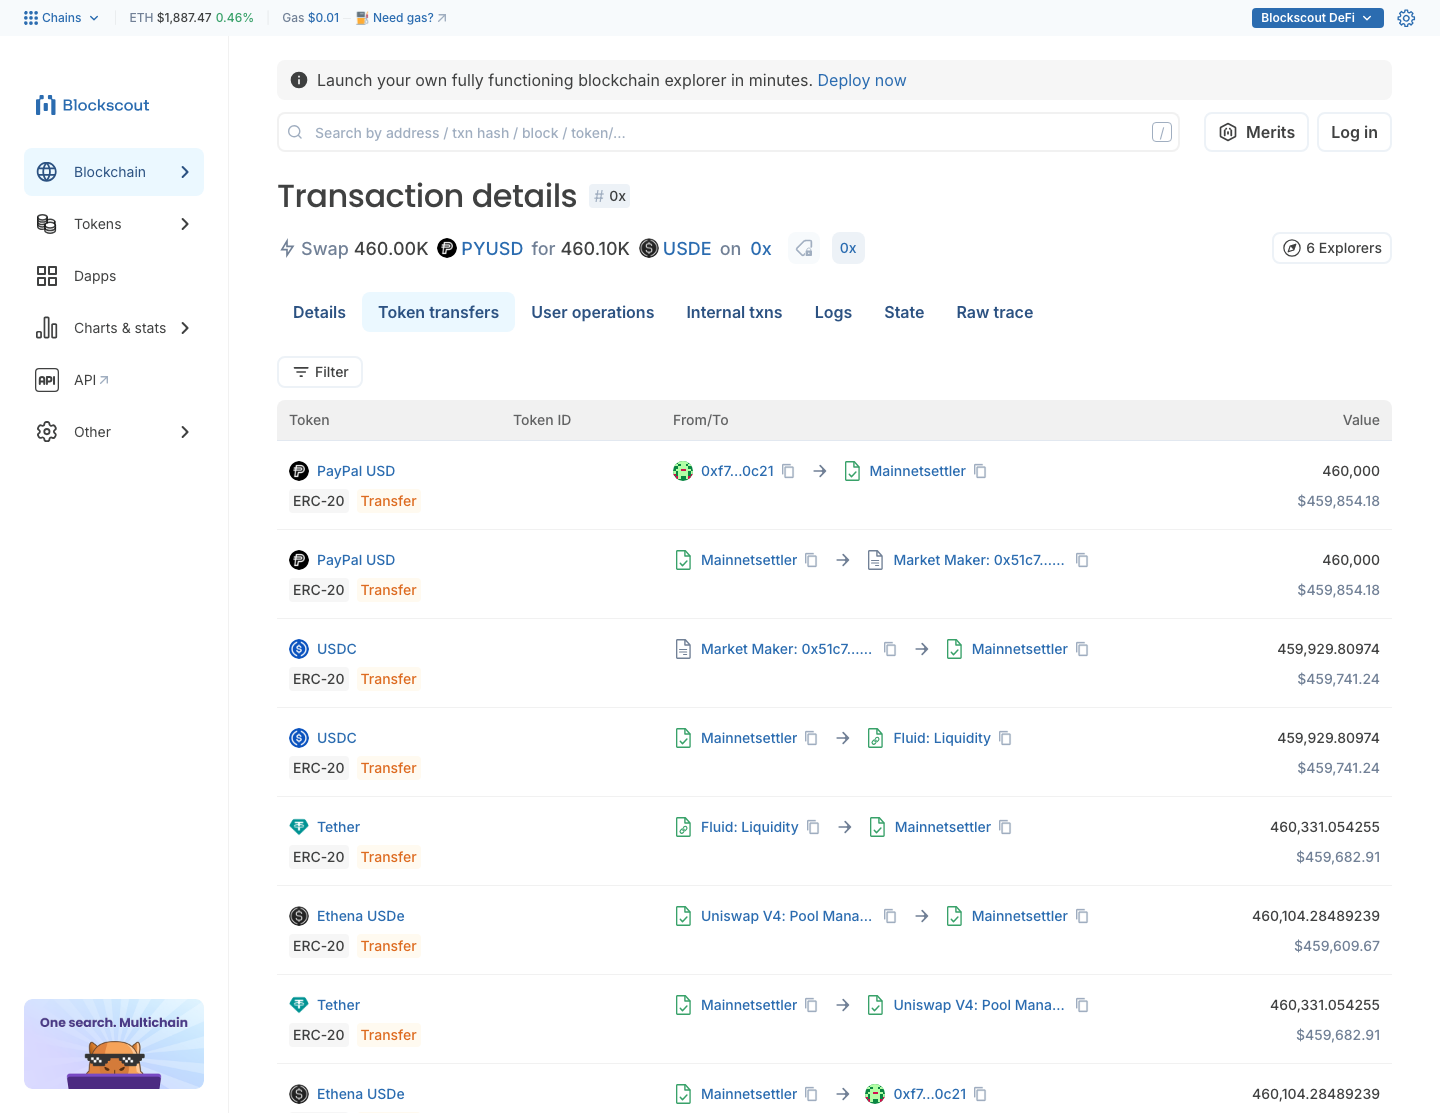
\includegraphics[width=0.88\textwidth,height=1.38cm,keepaspectratio,trim=270 820 430 170,clip]{assets/observed_route_blockscout.png}}
\par\vspace{0.15cm}
\evidencekicker{The decisive settlement transfers}
\vspace{0.02cm}
\fcolorbox{rule}{white}{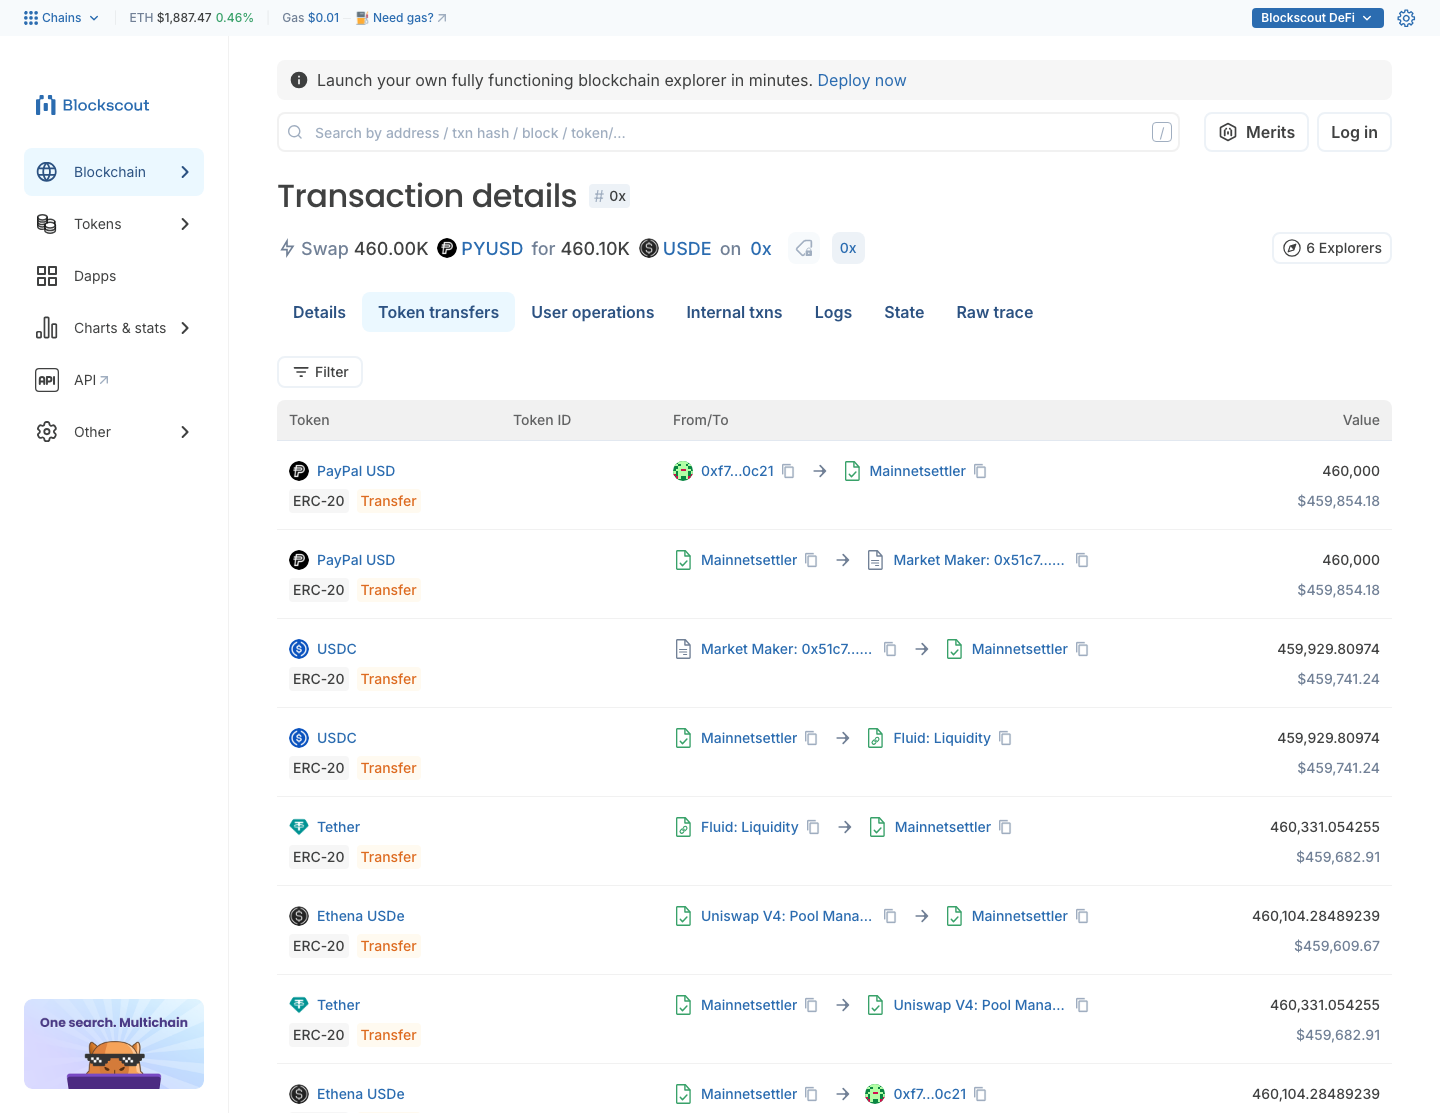
\includegraphics[width=0.94\textwidth,height=1.04cm,keepaspectratio,trim=280 415 324 615,clip]{assets/observed_route_blockscout.png}}
\par\vspace{0.08cm}
\fcolorbox{rule}{white}{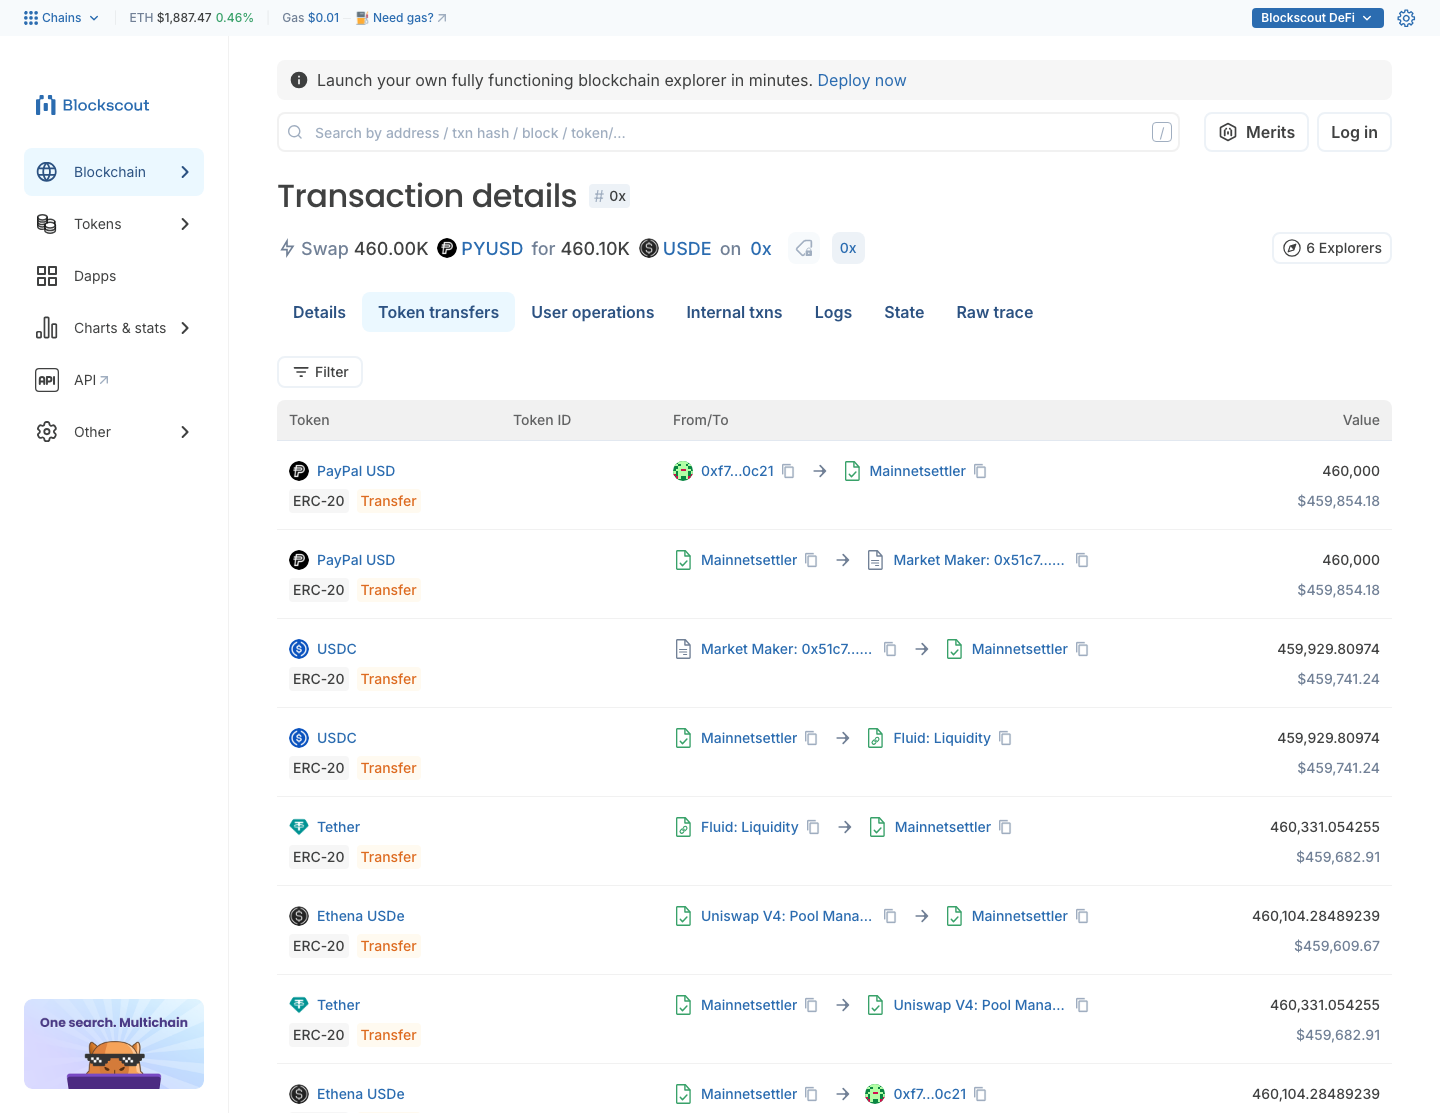
\includegraphics[width=0.94\textwidth,height=1.04cm,keepaspectratio,trim=280 320 324 700,clip]{assets/observed_route_blockscout.png}}
\par\vspace{0.14cm}
{\normalsize\raggedright The instruction is PYUSD $\rightarrow$ USDe. The maker supplies the USDC used by the Fluid leg, which begins the connected pool route.\par}
\decknote{The explorer screenshot and transfer trace refer to transaction \ethtx{0xbda1d07f17c503b5a9c8117c5d1383472006af8a9e22aa4e5e30804b9bf67ad9}{0xbda1d07f\ldots 9bf67ad9} on 10 January 2026.}
\end{frame}

% EVIDENCE-STATUS: authentic connected pool-swap component from the same transaction; exact same-state alternative remains outside this exhibit
% EVIDENCE-COMMIT: ab2c76231653b447c7b151b8d9b4a3fdd7b413e8
% EVIDENCE-SOURCES: output/exhibits/route_replay.json; data/unified/20260110.parquet
% EVIDENCE-GENERATION: transaction 0xbda1d07f17c503b5a9c8117c5d1383472006af8a9e22aa4e5e30804b9bf67ad9 component 0; partition sha256 a6870bc64badeecf030a1096e69b2ddfc9202e5c4ef99a8c5237d4d458033c6d
% VISUAL-FUNCTION: observed vehicle use | source-versus-pool-route breadcrumb plus native connected-route diagram | define the component endpoints and intermediary used in the vehicle-dominance measure
\begin{frame}{Inside the pools, USDT links USDC to USDe}
\centering
\vspace{-0.05cm}
\evidencekicker{Ordered transfers and route reconstruction}
\vspace{0.06cm}
\begin{tikzpicture}[x=1cm,y=1cm]
\node[softbox,inner sep=4pt,text width=3.35cm,minimum height=0.58cm,align=center] (user) at (2.75,0) {\scriptsize User instruction: PYUSD $\rightarrow$ USDe};
\node[font=\small\bfseries,text=muted] at (5.20,0) {$\Longrightarrow$};
\node[softbox,inner sep=4pt,draw=stable,text width=4.15cm,minimum height=0.58cm,align=center] (pools) at (8.30,0) {\scriptsize Pool route: USDC $\rightarrow$ USDT $\rightarrow$ USDe};
\end{tikzpicture}
\vspace{0.20cm}
\begin{tikzpicture}[x=1cm,y=1cm]
\node[nodepoint,minimum size=46pt,font=\small\bfseries] (a) at (1.30,3.25) {USDC};
\node[nodepoint,fill=ucldark,text=white,draw=ucldark,minimum size=46pt,font=\small\bfseries] (k) at (6.15,3.25) {USDT};
\node[nodepoint,minimum size=46pt,font=\small\bfseries] (b) at (11.00,3.25) {USDe};
\draw[route,draw=ucldark,line width=1.8pt] (a)--(k);
\draw[route,draw=ucldark,line width=1.8pt] (k)--(b);
\node[font=\normalsize\bfseries,text=ucldark,align=center] at (3.72,4.18) {Fluid};
\node[font=\normalsize\bfseries,text=ucldark,align=center] at (8.57,4.18) {Uniswap V4};
\node[font=\small,text=muted,align=center] at (3.72,2.31) {\RouteReplayInputAmount{} USDC\\$\rightarrow$ \RouteReplayVehicleAmount{} USDT};
\node[font=\small,text=muted,align=center] at (8.57,2.31) {\RouteReplayVehicleAmount{} USDT\\$\rightarrow$ \RouteReplayOutputAmount{} USDe};
\node[font=\scriptsize\bfseries,text=white,fill=ucldark,rounded corners=2pt,inner sep=4pt] at (6.15,1.15) {vehicle};
\end{tikzpicture}
\vspace{0.15cm}
\begin{minipage}{0.78\textwidth}
\centering
{\small Our route sample begins with USDC, the source asset of the connected pool-swap component. USDT is the vehicle because it links the two legs.\par}
\end{minipage}
\par\vspace{0.04cm}
{\raggedright\decknote{The route is the connected pool-swap component of transaction \ethtx{0xbda1d07f17c503b5a9c8117c5d1383472006af8a9e22aa4e5e30804b9bf67ad9}{0xbda1d07f\ldots 9bf67ad9} on 10 January 2026.}}
\end{frame}

% VISUAL-FUNCTION: dominance denominator | route glyph plus paired measure definitions | separate count, value, and network position
\begin{frame}{Vehicle dominance is the share of indirect trade carried by an asset}
\begin{columns}[T,totalwidth=\textwidth]
\begin{column}{0.43\textwidth}
\evidencekicker{Measurement}
\begin{itemize}
\item Dominance is the share of indirect trade intermediated by asset $k$.
\item Count share treats each route equally; value share weights routes by dollar value.
\item Network measures capture how broadly $k$ connects endpoint pairs.
\end{itemize}
\end{column}
\begin{column}{0.53\textwidth}
\centering
\begin{tikzpicture}[x=1cm,y=1cm]
\node[nodepoint] (a) at (0,3.45) {$i$};
\node[nodepoint,fill=ucldark,text=white,draw=ucldark] (k) at (2.0,3.45) {$k$};
\node[nodepoint] (b) at (4.0,3.45) {$o$};
\draw[route] (a) -- (k);
\draw[route] (k) -- (b);
\node[anchor=west,font=\small\bfseries,text=ucldark] at (0,2.10) {Count-weighted dominance};
\node[anchor=west,font=\small,align=left,text width=6.0cm] at (0,1.58) {Share of indirect routes that pass through $k$};
\node[anchor=west,font=\small\bfseries,text=stable] at (0,0.78) {Value-weighted dominance};
\node[anchor=west,font=\small,align=left,text width=6.0cm] at (0,0.26) {Share of comparable routed value that passes through $k$};
\end{tikzpicture}
\end{column}
\end{columns}
\end{frame}

% EVIDENCE-STATUS: verified institutional mechanism; no empirical estimate is displayed.
% SOURCE-GENERATION: repository HEAD eac25258ea36.
% SOURCE: docs/finding-v1-forced-vehicle.md sha256=650004eafae8864fe13b3d90ab59daefd77b342e33510f3d5db03b3e28ed2c68 (V1/V2 pairing contract).
% SOURCE: literature/text/2021-AdamsZinsmeisterRobinson2021UniswapV3-whitepaper-uniswap-v3-core.txt sha256=599a20254f8d5f1d6e771d2899bf16e4a921c5bc3a9cb82e58c97d7791411567 (V3 ranges, ticks, and fee tiers).
% SOURCE: https://app.uniswap.org/whitepaper-v4.pdf, Adams et al. (2024), Uniswap v4 Core, Sections 1 and 3 (singleton, hooks, and flash accounting).
% SOURCE: docs/research-questions-and-empirical-design.md sha256=b56cb5e98d93d0968306fc2dd36edb323d83519daab17b5c7b39587d49506c8b (V4 settlement boundary).
% SOURCE: src/ddvc/execution_contracts.py sha256=67b28ca58519cf9cef80314211f168989b60502c5a3fb8792ad8814613ddae00 (supported V4 vanilla concentrated-liquidity contract).
% SCIENTIFIC-BOUNDARY: architecture changes feasible pair formation, liquidity placement, or settlement. Pool adoption and realised route use are endogenous exposure, and calendar date alone is not treatment.
% VISUAL-FUNCTION: V1-to-V4 architecture morph | four-panel mechanism strip | separate design, realised exposure, and calendar time
\begin{frame}{Architecture changes routing opportunities}
\setlength{\fboxsep}{5pt}
\setlength{\fboxrule}{0.45pt}
\begin{columns}[T,totalwidth=\textwidth]

% V1: the pairing contract makes ETH the only token-to-token path.
\begin{column}{0.238\textwidth}
\fcolorbox{rule}{panel}{\begin{minipage}[t][3.95cm][t]{0.88\linewidth}
{\small\bfseries\color{ucldark}V1}\hfill{\scriptsize\color{muted}mandatory hub}\par
\vspace{0.18cm}
\centering
\begin{tikzpicture}[tinyasset/.style={circle,draw=ink,fill=white,minimum size=14pt,inner sep=0pt,font=\tiny},routearrow/.style={-{Stealth[length=4pt]},line width=1.15pt}]
\node[tinyasset] (a) at (0,0) {A};
\node[tinyasset,fill=ucldark,text=white,draw=ucldark,minimum size=23pt] (k) at (1.05,0) {ETH};
\node[tinyasset] (b) at (2.10,0) {B};
\draw[routearrow,draw=accent] (a)--(k);
\draw[routearrow,draw=accent] (k)--(b);
\draw[rule,densely dashed] (a) to[bend left=35] node[above,font=\tiny,text=muted] {no direct pool} (b);
\end{tikzpicture}
\par\vspace{0.22cm}
\raggedright\scriptsize Only ETH--token pools: token-to-token execution must pass through ETH.\par
\vfill
{\scriptsize\bfseries\color{accent}Hub use is imposed}\par
\end{minipage}}
\end{column}

% V2: arbitrary pairs add a direct opportunity while leaving vehicle routes feasible.
\begin{column}{0.238\textwidth}
\fcolorbox{rule}{panel}{\begin{minipage}[t][3.95cm][t]{0.88\linewidth}
{\small\bfseries\color{ucldark}V2}\hfill{\scriptsize\color{muted}pair choice}\par
\vspace{0.18cm}
\centering
\begin{tikzpicture}[tinyasset/.style={circle,draw=ink,fill=white,minimum size=14pt,inner sep=0pt,font=\tiny},routearrow/.style={-{Stealth[length=4pt]},line width=1.15pt}]
\node[tinyasset] (a) at (0,0) {A};
\node[tinyasset,fill=ucldark,text=white,draw=ucldark,minimum size=23pt] (k) at (1.05,0) {$k$};
\node[tinyasset] (b) at (2.10,0) {B};
\draw[routearrow,draw=ucldark] (a)--(k);
\draw[routearrow,draw=ucldark] (k)--(b);
\draw[routearrow,draw=stable] (a) to[bend left=35] node[above,font=\tiny,text=stable] {direct} (b);
\end{tikzpicture}
\par\vspace{0.22cm}
\raggedright\scriptsize Arbitrary pairs add a direct route; vehicle routes remain feasible.\par
\vfill
{\scriptsize\bfseries\color{stable}Hub use becomes a choice}\par
\end{minipage}}
\end{column}

% V3: bounded ranges make active depth depend on where liquidity is placed.
\begin{column}{0.238\textwidth}
\fcolorbox{rule}{panel}{\begin{minipage}[t][3.95cm][t]{0.88\linewidth}
{\small\bfseries\color{ucldark}V3}\hfill{\scriptsize\color{muted}range choice}\par
\vspace{0.25cm}
\centering
\begin{tikzpicture}[x=1cm,y=1cm]
\node[anchor=east,font=\tiny] at (0.28,0.27) {A/B};
\draw[rule,line width=0.85pt] (0.38,0.27)--(2.18,0.27);
\draw[stable,line width=3pt] (0.83,0.27)--(1.35,0.27);
\node[anchor=east,font=\tiny] at (0.28,-0.20) {via $k$};
\draw[rule,line width=0.85pt] (0.38,-0.20)--(2.18,-0.20);
\draw[ucldark,line width=3pt] (0.58,-0.20)--(1.08,-0.20);
\draw[uclbright,line width=3pt] (1.48,-0.20)--(2.02,-0.20);
\end{tikzpicture}
\par\vspace{0.28cm}
\raggedright\scriptsize LPs choose ranges and fees; active depth can favor direct pairs or vehicle spokes.\par
\vfill
{\scriptsize\bfseries\color{uclbright}Opportunity shifts by pair}\par
\end{minipage}}
\end{column}

% V4: settlement can net movement without erasing the economic route or its pools.
\begin{column}{0.238\textwidth}
\fcolorbox{rule}{panel}{\begin{minipage}[t][3.95cm][t]{0.88\linewidth}
{\small\bfseries\color{ucldark}V4}\hfill{\scriptsize\color{muted}net settlement}\par
\vspace{0.18cm}
\centering
\begin{tikzpicture}[tinyasset/.style={circle,draw=ink,fill=white,minimum size=14pt,inner sep=0pt,font=\tiny},routearrow/.style={-{Stealth[length=4pt]},line width=1.15pt}]
\node[rounded corners=2pt,draw=uclbright,densely dashed,minimum width=2.45cm,minimum height=0.92cm] at (1.05,0) {};
\node[tinyasset] (a) at (0,0) {A};
\node[tinyasset,fill=ucldark,text=white,draw=ucldark,minimum size=21pt] (k) at (1.05,0) {$k$};
\node[tinyasset] (b) at (2.10,0) {B};
\draw[routearrow,draw=ucldark] (a)--(k);
\draw[routearrow,draw=ucldark] (k)--(b);
\node[anchor=north,font=\tiny,text=uclbright] at (1.05,-0.50) {shared accounting};
\end{tikzpicture}
\par\vspace{0.22cm}
\raggedright\scriptsize Two pools still execute; intermediate token movement may be netted.\par
\vfill
{\scriptsize\bfseries\color{ucldark}Settlement can diverge from route use}\par
\end{minipage}}
\end{column}
\end{columns}

% The empirical design must not substitute the version date for exposure to its mechanism.
\vspace{0.25cm}
\colorbox{panel}{\parbox[c][0.72cm][c]{0.965\textwidth}{\hspace{0.15cm}\scriptsize
\textbf{Architecture}\; feasible rules\hfill
\textbf{Exposure}\; realised pool and route use\hfill
\textbf{Calendar date}\; timing only\hspace{0.15cm}}}
\end{frame}

% VISUAL-MANAGED-FILE
% The former route-sample-versus-supplement frame was removed from the
% talk. Economic objects and protocol mechanisms are introduced where used;
% the appendix retains the detailed measurement and architecture material.
% RETAINED SCOPE CONTRACT: Main route sample = Uniswap v1/v2/v3/v4, SushiSwap v2/v3, Curve, Balancer, and Fluid.
% RETAINED SCOPE CONTRACT: The V1/V2 architecture supplement isolates the venue rule within that shared route panel.

% Mechanisms and estimands. Sources: docs/specification-lock.json and docs/research-workflow.md.

\begin{frame}{Four forces can sustain vehicle dominance}
\begin{center}
\begin{tikzpicture}[scale=0.98,transform shape]
\node[nodepoint,fill=ucldark,text=white,draw=ucldark,minimum size=46pt,font=\normalsize\bfseries,align=center] (d) at (0,0) {vehicle\\dominance};
\node[softbox,minimum width=3.15cm,align=center] (liq) at (-4.15,2.15) {\textbf{Liquidity provision}\\capital follows order flow};
\node[softbox,minimum width=3.15cm,align=center] (def) at (4.15,2.15) {\textbf{Coordination}\\pairs and defaults persist};
\node[softbox,minimum width=3.15cm,align=center] (int) at (-4.15,-2.15) {\textbf{Market integration}\\more routes become reachable};
\node[softbox,minimum width=3.15cm,align=center] (hold) at (4.15,-2.15) {\textbf{Holding cost}\\volatility and backing differ};
\draw[route,draw=native] (liq)--(d);
\draw[route,draw=uclbright] (def)--(d);
\draw[route,draw=stable] (int)--(d);
\draw[route,draw=imported] (hold)--(d);
\end{tikzpicture}
\end{center}
\vspace{0.2cm}
{\small The design measures each force separately before asking which one accounts for changes in dominance.\par}
\end{frame}

\begin{frame}{The empirical design separates formation, rotation, and persistence}
\begin{columns}[T]
\begin{column}{0.30\textwidth}
\evidencekicker{Formation}
\textbf{Architecture changes}\par
Imposed intermediation, arbitrary pairing, concentrated liquidity, and singleton settlement.
\end{column}
\begin{column}{0.30\textwidth}
\evidencekicker{Rotation}
\textbf{Panel variation}\par
Count share, value share, excess use, network position, and route complexity over time.
\end{column}
\begin{column}{0.30\textwidth}
\evidencekicker{Persistence}
\textbf{Exact alternatives}\par
The role can be observed while another feasible route is cheaper at the same state.
\end{column}
\end{columns}
\vspace{0.75cm}
\begin{tikzpicture}
\draw[route,draw=rule,line width=2pt] (0,0) -- (11.8,0);
\fill[ucldark] (0.7,0) circle (3pt);
\fill[stable] (5.9,0) circle (3pt);
\fill[accent] (11.1,0) circle (3pt);
\node[below,font=\small] at (0.7,-0.15) {how the role begins};
\node[below,font=\small] at (5.9,-0.15) {how its share moves};
\node[below,font=\small] at (11.1,-0.15) {how long it survives};
\end{tikzpicture}
\end{frame}

% EVIDENCE-MANAGED-FILE
% VISUAL-MANAGED-FILE
% Numerical cells are generated; evidence status and identities stay in comments.
\IfFileExists{../output/exhibits/provisional_results_deck_values.tex}{%
% Generated by scripts/tabulate/render_provisional_results_deck_values.py.
% PROVISIONAL working-paper values; scientific identity is recorded in the provenance sidecar.
\newcommand{\StableCountBase}{16.9\%}
\newcommand{\StableCountEnd}{42.3\%}
\newcommand{\StableCountChange}{$+25.4$ pp}
\newcommand{\StableCountSE}{1.05 pp}
\newcommand{\StableCountP}{$3.35\times10^{-87}$}
\newcommand{\StableValueBase}{32.7\%}
\newcommand{\StableValueEnd}{76.5\%}
\newcommand{\StableValueChange}{$+43.9$ pp}
\newcommand{\StableValueSE}{2.02 pp}
\newcommand{\StableValueP}{$4.46\times10^{-75}$}
\newcommand{\MultiLegCountBase}{44.5\%}
\newcommand{\MultiLegCountEnd}{60.7\%}
\newcommand{\MultiLegCountChange}{$+16.3$ pp}
\newcommand{\MultiLegCountSE}{1.86 pp}
\newcommand{\MultiLegValueBase}{47.3\%}
\newcommand{\MultiLegValueEnd}{83.2\%}
\newcommand{\MultiLegValueChange}{$+35.9$ pp}
\newcommand{\MultiLegValueSE}{1.68 pp}
\newcommand{\WeakestComplexityCountChange}{$+17.0$ pp}
\newcommand{\WeakestComplexityCountSE}{1.36 pp}
\newcommand{\WeakestComplexityValueChange}{$+25.6$ pp}
\newcommand{\WeakestComplexityValueSE}{1.52 pp}
\newcommand{\JointStableContribution}{92.1\%}
\newcommand{\USDTCountExcessBase}{1.06}
\newcommand{\USDTCountExcessEnd}{1.23}
\newcommand{\USDTValueExcessBase}{0.59}
\newcommand{\USDTValueExcessEnd}{1.42}
\newcommand{\USDTCrossCountChange}{$+7.59$ pp}
\newcommand{\USDTCrossCountSE}{0.88 pp}
\newcommand{\USDTCrossValueChange}{$+12.00$ pp}
\newcommand{\USDTCrossValueSE}{2.03 pp}
\newcommand{\USDTEndpointGapBase}{$-7.13$ pp}
\newcommand{\USDTEndpointGapEnd}{$+8.14$ pp}
\newcommand{\USDTEndpointGapChange}{$+15.27$ pp}
\newcommand{\USDTEndpointGapSE}{1.50 pp}
\newcommand{\FullIntermediationBase}{13.95\%}
\newcommand{\FullIntermediationEnd}{11.92\%}
\newcommand{\FullIntermediationChange}{$-2.03$ pp}
\newcommand{\FullIntermediationSE}{0.39 pp}
\newcommand{\BalancedIntermediationEnd}{8.60\%}
\newcommand{\BalancedIntermediationChange}{$-5.35$ pp}
\newcommand{\BalancedIntermediationSE}{0.38 pp}
\newcommand{\CrossVenueCountStart}{2.0\%}
\newcommand{\CrossVenueCountEnd}{57.2\%}
\newcommand{\CrossVenueValueEnd}{79.1\%}
\newcommand{\CrossVenueRotationPremium}{$+7.45$ pp}
\newcommand{\CrossVenueRotationSE}{1.33 pp}
\newcommand{\VenueAllStableCountBase}{1.27}
\newcommand{\VenueAllStableCountEnd}{1.41}
\newcommand{\VenueAllStableValueBase}{0.84}
\newcommand{\VenueAllStableValueEnd}{1.24}
\newcommand{\VenueCPStableCountBase}{1.28}
\newcommand{\VenueCPStableCountEnd}{1.42}
\newcommand{\VenueCPStableValueBase}{0.78}
\newcommand{\VenueCPStableValueEnd}{1.33}
\newcommand{\VenueCPNativeValueEnd}{0.62}
\newcommand{\VenueAllStableValueChange}{$+0.40$}
\newcommand{\VenueCPStableValueChange}{$+0.55$}
\newcommand{\VenueCPEpisodeShare}{84.8\%}
\newcommand{\VenueBalancerPeakEpisodes}{39,536}
\newcommand{\VenueCPPeakEpisodes}{8,767,213}
\newcommand{\RouterWindowDays}{60}
\newcommand{\RouterReleaseCount}{3}
\newcommand{\RouterIntermediationBase}{20.8\%}
\newcommand{\RouterIntermediationEnd}{12.5\%}
\newcommand{\RouterIntermediationOne}{$-5.7$ pp}
\newcommand{\RouterIntermediationTwo}{$+0.8$ pp}
\newcommand{\RouterIntermediationThree}{$-0.7$ pp}
\newcommand{\RouterLargestIntermediationRise}{$+0.8$ pp}
\newcommand{\RouterLargestLegMovement}{0.049}
\newcommand{\RouterCrossBase}{8.5\%}
\newcommand{\RouterCrossOne}{$+2.5$ pp}
\newcommand{\RouterCrossTwo}{$+3.1$ pp}
\newcommand{\RouterCrossThree}{$-2.0$ pp}
\newcommand{\RouterCrossEnd}{24.4\%}
%
}{}
\IfFileExists{../output/exhibits/vehicle_transition_pair_decomposition_deck_values.tex}{%
% Generated by scripts/build_vehicle_transition_pair_deck_values.py; do not edit.
\newcommand{\PairPooledBase}{16.9\%}
\newcommand{\PairPooledEnd}{42.5\%}
\newcommand{\PairPooledTotal}{+25.7\,pp}
\newcommand{\PairPooledReweight}{+8.6\,pp}
\newcommand{\PairPooledSupportMass}{-0.5\,pp}
\newcommand{\PairPooledExclusive}{+17.8\,pp}
\newcommand{\PairPooledWithin}{-0.1\,pp}
\newcommand{\PairPooledBaseRawPct}{16.865562569}
\newcommand{\PairPooledEndRawPct}{42.540936227}
\newcommand{\PairPooledReweightRawPP}{8.572531324}
\newcommand{\PairPooledSupportMassRawPP}{-0.536299548}
\newcommand{\PairPooledExclusiveRawPP}{17.767073765}
\newcommand{\PairPooledWithinRawPP}{-0.127931883}
\newcommand{\PairSingleTotal}{+21.1\,pp}
\newcommand{\PairSingleWithin}{-0.3\,pp}
\newcommand{\PairCrossTotal}{+31.4\,pp}
\newcommand{\PairCrossWithin}{-0.3\,pp}
\newcommand{\PairValueTotal}{+42.8\,pp}
\newcommand{\PairValueWithin}{0.0\,pp}
\newcommand{\PairValueReweight}{+26.2\,pp}
\newcommand{\PairValueSupportMass}{-2.5\,pp}
\newcommand{\PairValueExclusive}{+19.2\,pp}
%
}{\PackageError{dvc-deck}{Missing generated vehicle-pair decomposition values}{Run scripts/build_vehicle_transition_pair_deck_values.py.}}
\IfFileExists{../output/exhibits/v1_architecture_deck_values.tex}{%
% Generated presentation binding for the admitted V1/V2 architecture result.
% Source: docs/finding-v1-forced-vehicle.md at ebeb23cf56b15dc78d798ea5770976560384a6d0.
% The regression in tests/test_deck_evidence.py reopens these bindings against
% the source tables whenever either file changes.
\newcommand{\VOneForcedRoutes}{217,003}
\newcommand{\VTwoWethTradeShare}{95.5\%}
\newcommand{\VTwoWethNewPairShare}{97.9\%}
%
}{\PackageError{dvc-deck}{Missing generated V1/V2 architecture values}{Rebuild the admitted V1/V2 presentation binding.}}

% EVIDENCE-STATUS: evolving route result; current certified route release
% EVIDENCE-COMMIT: 2ffbce0
% EVIDENCE-SOURCES: output/figures/experiments/annual_vehicle_composition_bands.pdf; output/exhibits/intermediation_by_type.jsonl; docs/findings-freeze.md
% VISUAL-FUNCTION: non-monotone realised vehicle rotation | annual native/stable lead comparison separated by count/value | expose the value lead-loss-retake path without implying treatment
\begin{frame}{Stablecoins regain the lead in routed value}
\vspace{-0.05cm}
\begin{center}
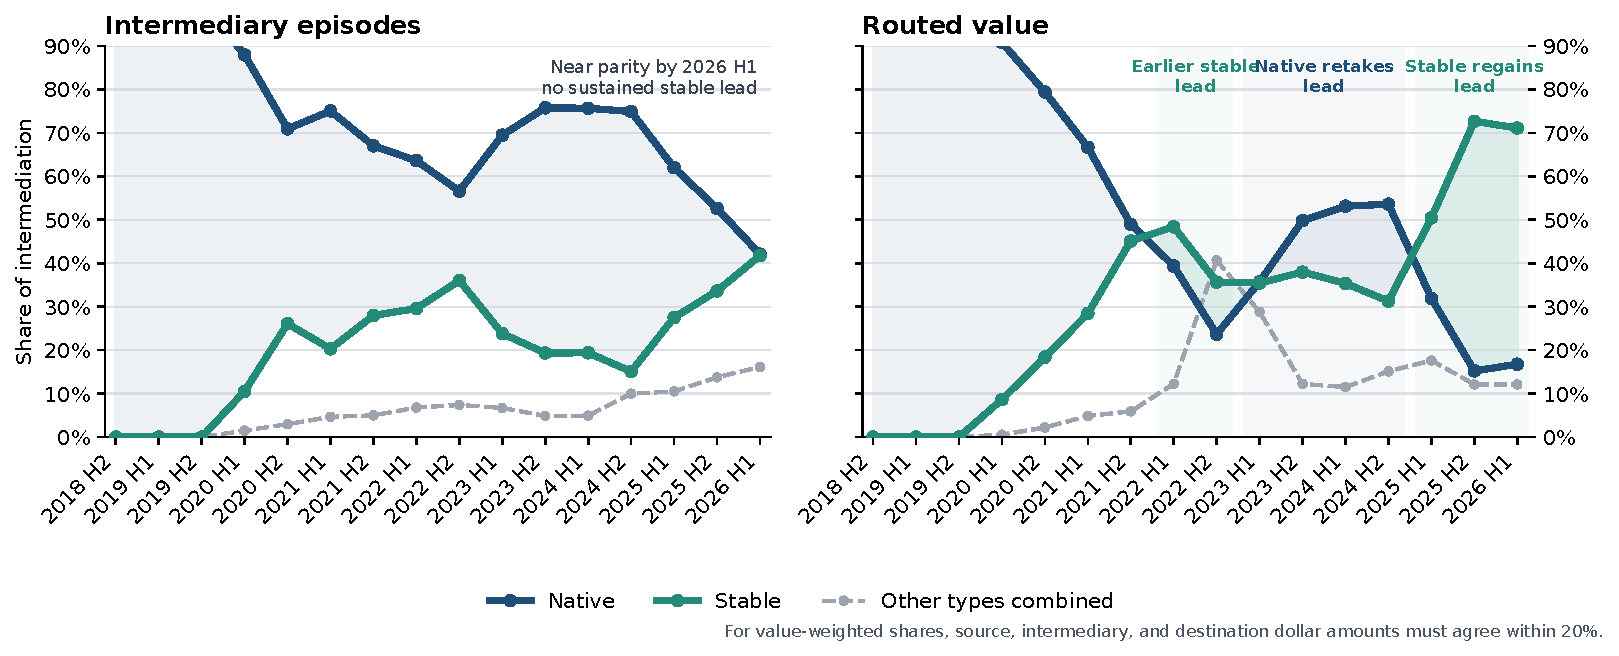
\includegraphics[width=0.94\textwidth,height=0.69\textheight,keepaspectratio]{../output/figures/experiments/annual_vehicle_composition_bands.pdf}
\end{center}
\vspace{-0.14cm}
\decknote{Annual shares of observed vehicle routes. The 2026 observation covers January--June; Other combines imported, liquid-staking, and residual assets.}
\end{frame}

% EVIDENCE-STATUS: evolving route decomposition; venue-scope reweighting is a route-only descriptive identity
% EVIDENCE-COMMIT: 6dd7897
% EVIDENCE-SOURCES: output/figures/vehicle_excess_use_transition.pdf; output/exhibits/vehicle_excess_use.jsonl; output/exhibits/vehicle_excess_use_transition.jsonl; output/exhibits/e0_usdt_integration_decomposition.jsonl; docs/findings-freeze.md
% VISUAL-FUNCTION: candidate-level excess-use change | paired count/value dumbbells | identify the distinct USDT contribution
\begin{frame}{USDT drives the rise in stablecoin intermediation}
\vspace{-0.08cm}
\begin{center}
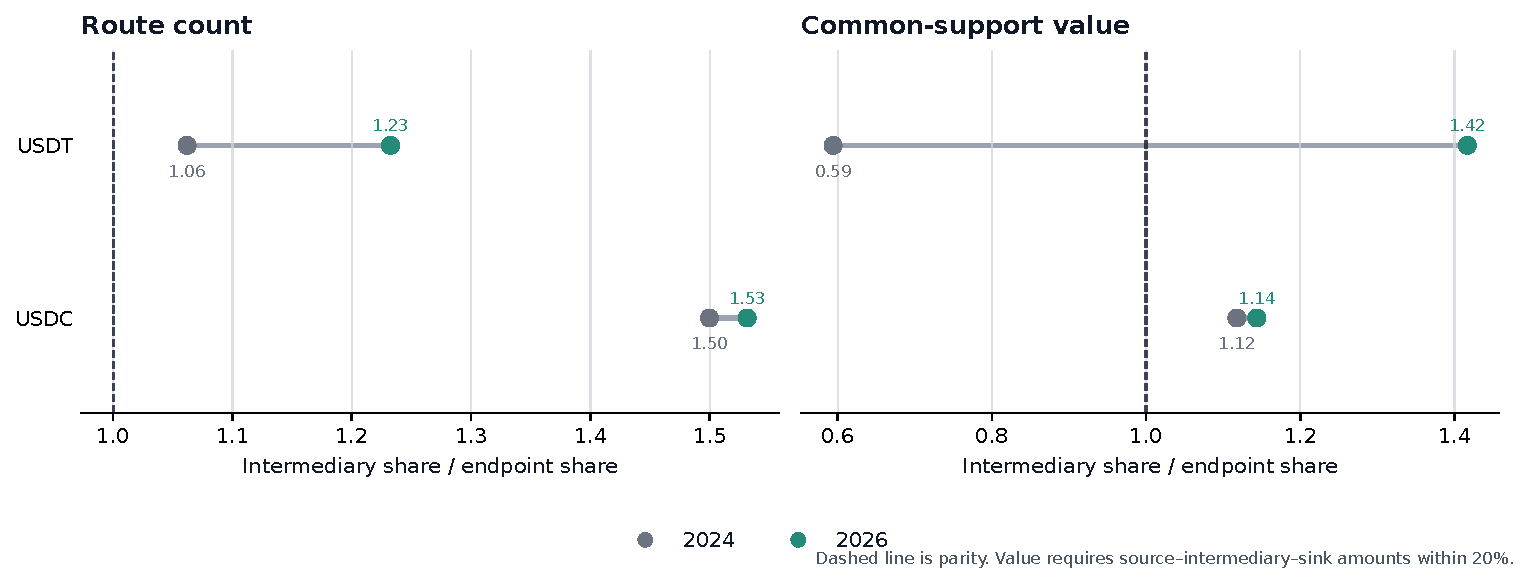
\includegraphics[width=0.93\textwidth,height=0.44\textheight,keepaspectratio]{../output/figures/vehicle_excess_use_transition.pdf}
\end{center}
\vspace{-0.16cm}
{\fontsize{6.8}{7.5}\selectfont USDT crosses parity by routed value and extends its count advantage; USDC changes little.}
\vspace{0.04cm}
\begin{beamercolorbox}[sep=0.08cm,wd=\textwidth]{block body}
{\fontsize{7.0}{7.7}\selectfont\bfseries \USDTVenueWithinCountShare{} of the count-share change and \USDTVenueWithinValueShare{} of the routed-value change occur within the single- and cross-venue categories.}
\end{beamercolorbox}
\decknote{Excess use is intermediary share divided by endpoint share on the same route perimeter. The comparison uses the same January--June dates in 2024 and 2026.}
\end{frame}

% EVIDENCE-STATUS: certified descriptive route accounting and matched-market estimate; mechanism remains open
% EVIDENCE-COMMIT: b21ed0a
% EVIDENCE-PRODUCER-COMMIT: 0f90441
% EVIDENCE-SOURCES: output/exhibits/vehicle_transition_pair_decomposition.jsonl; output/exhibits/vehicle_transition_pair_support.jsonl; output/exhibits/vehicle_transition_pair_fixed_effects.jsonl; output/exhibits/vehicle_transition_pair_decomposition_deck_values.tex
% VISUAL-FUNCTION: five-factor composition plus matched-market confidence interval | native TikZ accounting ribbon and interval | distinguish observed pair support, activity, vehicle incidence, and within-market stable-share change
\begin{frame}{Pair activity and vehicle use: \PairAndVehicleShare{} of the gain}
\vspace{-0.34cm}
\begin{center}
\resizebox{0.93\textwidth}{!}{% Presentation geometry only. Numerical labels are generated in
% output/exhibits/route_methodology_heterogeneity_deck_values.tex.
% WETH is the native intermediary in this comparison. If WETH is an endpoint,
% it cannot also be the intermediary; every such row therefore has stable_share=1.
\begin{tikzpicture}[x=1cm,y=1cm]
\tikzset{panel/.style={draw=rule,fill=white,rounded corners=3pt,line width=0.8pt}}
\tikzset{small/.style={font=\fontsize{6.8}{7.5}\selectfont,text=muted,align=center}}

\node[draw=stable,line width=1.1pt,circle,minimum size=1.05cm,
  font=\fontsize{8.2}{8.8}\selectfont\bfseries,text=ucldark] at (1.05,3.45) {WETH};
\node[anchor=west,font=\fontsize{8.2}{9.0}\selectfont\bfseries,text=ucldark]
  at (1.82,3.62) {WETH is an endpoint of the ultimate pair};
\node[anchor=west,font=\fontsize{7.2}{8.0}\selectfont,text=ink]
  at (1.82,3.25) {Stablecoins alone remain eligible as intermediaries.};

\draw[panel] (0,0.56) rectangle (6.00,2.68);
\node[anchor=west,font=\fontsize{8.1}{8.8}\selectfont\bfseries,text=ucldark]
  at (0.35,2.32) {All matched ultimate-pair groups};
\node[anchor=west,font=\fontsize{23}{24}\selectfont\bfseries,text=stable]
  at (0.35,1.48) {\WethCountFullChange};
\node[anchor=west,font=\fontsize{6.9}{7.6}\selectfont,text=muted]
  at (0.35,1.05) {95\% CI [\WethCountFullCILower, \WethCountFullCIUpper]};
\node[anchor=west,font=\fontsize{7.0}{7.7}\selectfont,text=ink]
  at (0.35,0.80) {WETH-linked route-count mass: \WethCountMassBase{} $\rightarrow$ \WethCountMassEnd};

\draw[panel] (6.35,0.56) rectangle (12.35,2.68);
\node[anchor=west,font=\fontsize{8.1}{8.8}\selectfont\bfseries,text=ucldark]
  at (6.70,2.32) {Ultimate-pair groups excluding WETH endpoints};
\node[anchor=west,font=\fontsize{23}{24}\selectfont\bfseries,text=accent]
  at (6.70,1.48) {\WethCountNoEndpointChange};
\node[anchor=west,font=\fontsize{6.9}{7.6}\selectfont,text=muted]
  at (6.70,1.05) {95\% CI [\WethCountNoEndpointCILower, \WethCountNoEndpointCIUpper]};
\node[anchor=west,font=\fontsize{7.0}{7.7}\selectfont,text=ink]
  at (6.70,0.80) {\WethCountNoEndpointGroups{} matched groups};

\node[small,text width=12.0cm] at (6.18,0.08)
  {\textbf{Within-ultimate-pair change:} all groups \WethCountWithinFullChange{} [\WethCountWithinFullCILower, \WethCountWithinFullCIUpper];\\excluding WETH endpoints \WethCountWithinNoEndpointChange{} [\WethCountWithinNoEndpointCILower, \WethCountWithinNoEndpointCIUpper].};
\end{tikzpicture}
}
\end{center}
\vspace{-0.38cm}
{\fontsize{8.2}{9.1}\selectfont\textbf{Dollar-weighted routes show the same broad allocation.} Stable share rises \PairValueTotal, with \PairValueReweight\ from activity weights among continuing pairs and only \PairValueWithin\ from stable-for-native substitution within them.}

\vspace{0.02cm}
\decknote{The sample contains exact two-leg routes observed in 2024 and January--June 2026. Matched estimates compare the same ordered endpoint pair, calendar date, and single- versus cross-venue route category. Dollar-weighted calculations retain routes for which the source, intermediary, and destination dollar amounts agree within 20\%.}
\end{frame}

% EVIDENCE-STATUS: certified descriptive result; integration remains a selected route stratum
% EVIDENCE-COMMIT: a0c54e9
% EVIDENCE-SOURCES: output/figures/experiments/integration_change_forest.pdf; output/exhibits/intermediation_integration_rival.jsonl; output/exhibits/intermediation_integration_interaction.jsonl; docs/findings-freeze.md
% VISUAL-FUNCTION: integration-stratified vehicle rotation | change estimates with HAC intervals | test whether venue mix absorbs the stable-share change
\begin{frame}{Stablecoin use rises within each venue scope}
\vspace{-0.08cm}
\begin{center}
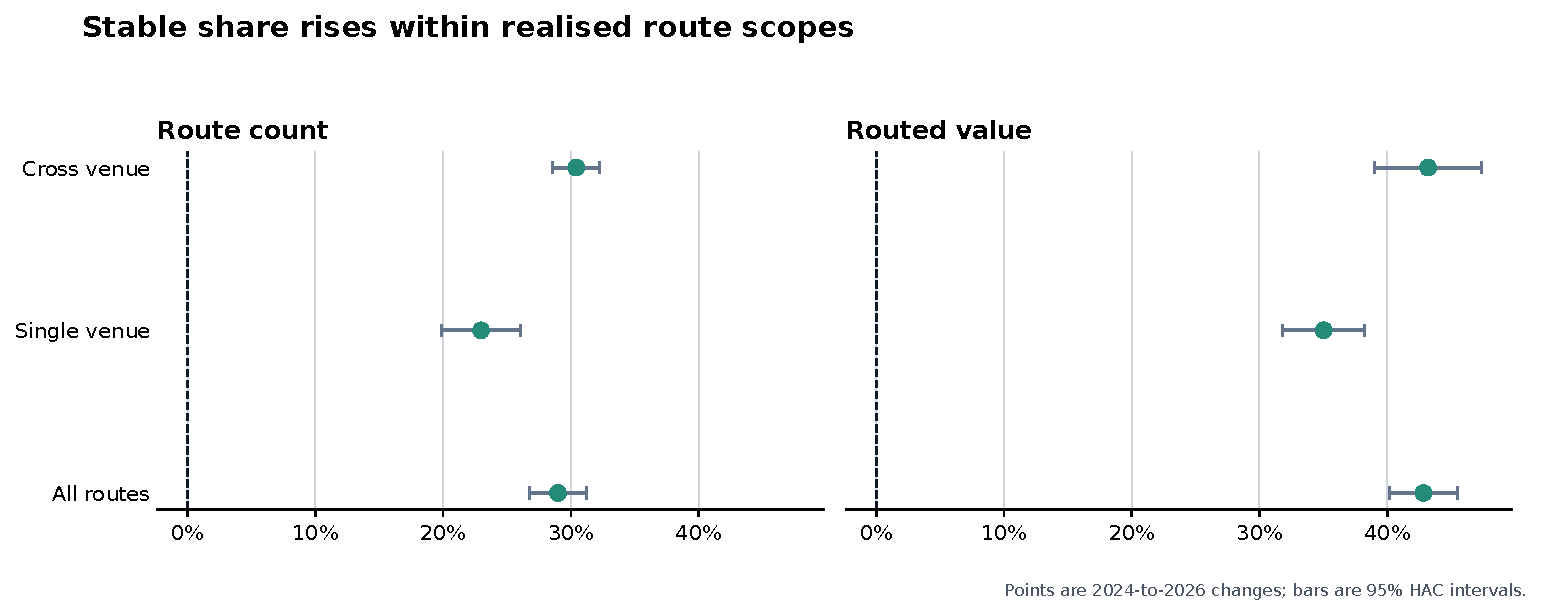
\includegraphics[width=0.89\textwidth,height=0.46\textheight,keepaspectratio]{../output/figures/experiments/integration_change_forest.pdf}
\end{center}
\vspace{-0.15cm}
{\fontsize{6.8}{7.5}\selectfont The increase appears within both realised route scopes, so a change in the single- versus cross-venue mix cannot account for the aggregate rotation. Cross-venue status remains selected; the comparison does not identify an effect of integration, routing software, or protocol architecture.}
\decknote{Changes compare the same January--June dates in 2024 and 2026. Bars show 95\% calendar-HAC confidence intervals.}
\end{frame}

% EVIDENCE-STATUS: registered mechanism design; no current LP estimate is displayed
% EVIDENCE-COMMIT: ab2c762
% EVIDENCE-SOURCES: docs/specification-lock.json; docs/findings-freeze.md; paper/sections/05-rivals.tex
% SCIENTIFIC-BOUNDARY: temporal ordering is not causal feedback; V2 capital stocks and V3 provider flows remain separate objects
% VISUAL-FUNCTION: liquidity timing test | two opposed timelines | distinguish capital-leading-use from use-leading-capital
\begin{frame}{Does liquidity move before vehicle use or follow it?}
\vspace{0.02cm}
\begin{columns}[T,totalwidth=\textwidth]
\begin{column}{0.48\textwidth}
\evidencekicker{Liquidity precedes use}
\vspace{0.25cm}
\centering
\begin{tikzpicture}[x=1cm,y=1cm]
\node[softbox,text width=4.35cm,minimum height=0.78cm,align=center] (capital) at (0,2.60) {More capital or provider inflow\\in vehicle-linked pools at $t$};
\node[softbox,text width=4.35cm,minimum height=0.78cm,align=center] (route) at (0,0.68) {More routes through the same vehicle\\at $t+\tau$};
\draw[-{Stealth[length=6pt]},line width=1.7pt,draw=stable] (capital)-- node[right,font=\scriptsize,text=muted] {predicts} (route);
\end{tikzpicture}
\par\vspace{0.10cm}\raggedright
{\small Liquidity supply may help a vehicle attract later routes.\par}
\end{column}
\begin{column}{0.48\textwidth}
\evidencekicker{Use precedes liquidity}
\vspace{0.25cm}
\centering
\begin{tikzpicture}[x=1cm,y=1cm]
\node[softbox,text width=4.35cm,minimum height=0.78cm,align=center] (route2) at (0,2.60) {More routes through a vehicle\\at $t$};
\node[softbox,text width=4.35cm,minimum height=0.78cm,align=center] (capital2) at (0,0.68) {More capital or provider inflow\\in its pools at $t+\tau$};
\draw[-{Stealth[length=6pt]},line width=1.7pt,draw=ucldark] (route2)-- node[right,font=\scriptsize,text=muted] {predicts} (capital2);
\end{tikzpicture}
\par\vspace{0.10cm}\raggedright
{\small Providers may instead follow routed demand.\par}
\end{column}
\end{columns}
\vspace{0.10cm}
{\fontsize{7.2}{8.0}\selectfont V2 capital stocks and V3 provider flows are tested separately at fixed lags; either ordering may reflect common demand or routing shocks.}
\end{frame}

% EVIDENCE-STATUS: registered V4 extension design; current estimate pending
% EVIDENCE-COMMIT: ab2c762
% EVIDENCE-SOURCES: docs/research-questions-and-empirical-design.md; docs/findings-freeze.md; paper/sections/05-rivals.tex
% SCIENTIFIC-BOUNDARY: settlement mechanics and route choice are distinct outcomes; launch date is not treatment
% VISUAL-FUNCTION: V4 settlement estimand | economic route versus physical transfer layers | show the matched comparison required to separate them
\begin{frame}{V4 separates the economic route from physical settlement}
\begin{columns}[T,totalwidth=\textwidth]
\begin{column}{0.48\textwidth}
\evidencekicker{Economic route}
\vspace{0.12cm}
\centering
\begin{tikzpicture}[x=1cm,y=1cm,tinyasset/.style={circle,draw=ink,fill=white,minimum size=23pt,inner sep=0pt,font=\small},routearrow/.style={-{Stealth[length=5pt]},line width=1.4pt}]
\node[tinyasset] (a) at (0,2.45) {A};
\node[tinyasset,fill=ucldark,text=white,draw=ucldark] (k) at (2.05,2.45) {$k$};
\node[tinyasset] (b) at (4.10,2.45) {B};
\draw[routearrow,draw=ucldark] (a)--(k);
\draw[routearrow,draw=ucldark] (k)--(b);
\node[anchor=north,align=center,font=\small,text width=5.2cm] at (2.05,1.82) {Pool calls route through intermediary $k$.};
\node[rounded corners=3pt,draw=uclbright,densely dashed,minimum width=5.0cm,minimum height=0.82cm,align=center,font=\scriptsize] at (2.05,0.45) {Prediction: fewer token transfers\\for comparable two-pool routes.};
\end{tikzpicture}
\end{column}
\begin{column}{0.05\textwidth}
\mbox{}
\end{column}
\begin{column}{0.44\textwidth}
\evidencekicker{Matched comparison}
\vspace{0.12cm}
{\scriptsize
\begin{itemize}
\setlength{\itemsep}{0.25em}
\item Compare routes in the same week, endpoint pair, intermediary, direction, and trade-size group.
\item Record route use and token transfers separately.
\item Compare feasible alternatives before interpreting vehicle choice.
\end{itemize}
}
\end{column}
\end{columns}
\end{frame}

% EVIDENCE-STATUS: diagnostic displacement gradient; not a persistence estimate
% EVIDENCE-COMMIT: 3873fca
% EVIDENCE-SOURCES: output/exhibits/provisional_results_deck_values.tex; docs/findings-freeze.md
% VISUAL-FUNCTION: 30-day challenger and incumbent share changes | coefficient table pending difference plot | expose direction, uncertainty, and risk-set limitation
\begin{frame}{Challenger cost advantage predicts subsequent vehicle share}
\vspace{0.18cm}
{\small
\begin{tabular}{@{}p{0.43\textwidth}rrr@{}}
\toprule
\textbf{30-day outcome} & $\hat\beta$ & \textbf{SE} & $t$ \\
\midrule
Change in challenger vehicle share & \ChallengerCoef & \ChallengerSE & \ChallengerT \\
Change in incumbent vehicle share & \IncumbentCoef & \IncumbentSE & \IncumbentT \\
Challenger leads after 30 days & \OvertakeCoef & \OvertakeSE & \OvertakeT \\
\bottomrule
\end{tabular}}
\vspace{0.25cm}

\decknote{$\hat\beta$ is the coefficient on the challenger's cost advantage. Outcomes are measured 30 days later. The sample contains $N=\DiagnosticN$ endpoint-pair--intermediary observations and \DiagnosticClusters\ date clusters; standard errors are clustered by date and use the CR1 rank correction.}
\vspace{0.36cm}
\begin{beamercolorbox}[sep=0.22cm,wd=\textwidth]{block body}
The estimates are large in the small set of endpoint markets and intermediary assets we can follow. They remain descriptive because the panel does not compare each market against a fixed set of feasible routes.
\end{beamercolorbox}
\end{frame}

% EVIDENCE-STATUS: admitted V1 mandate and V2 pair-formation result
% EVIDENCE-COMMIT: ebeb23c
% EVIDENCE-SOURCES: docs/finding-v1-forced-vehicle.md; output/exhibits/v1_forced_vehicle_report.md; output/exhibits/v1_architecture_deck_values.tex
% VISUAL-FUNCTION: architecture and persistence | V1-to-V2 mechanism comparison | show how imposed intermediation becomes endogenous pair formation
\begin{frame}{Native-asset pairing persists after it becomes optional}
\begin{columns}[T,totalwidth=\textwidth]
\begin{column}{0.43\textwidth}
\evidencekicker{V1: protocol rule}
\vspace{0.16cm}
\begin{tikzpicture}[x=1cm,y=1cm]
\node[nodepoint] (a) at (0.35,2.45) {A};
\node[nodepoint,fill=ucldark,text=white,draw=ucldark,minimum size=38pt] (eth) at (2.55,2.45) {ETH};
\node[nodepoint] (b) at (4.75,2.45) {B};
\draw[route,draw=accent,line width=1.7pt] (a)--(eth);
\draw[route,draw=accent,line width=1.7pt] (eth)--(b);
\node[font=\small\bfseries,text=ucldark,align=center] at (2.55,0.95) {\VOneForcedRoutes{} token-to-token trades\\pass through ETH};
\end{tikzpicture}
\vspace{0.10cm}
{\small Every token pool pairs with ETH, so the architecture imposes the vehicle.\par}
\end{column}
\begin{column}{0.08\textwidth}
\centering
\vspace{2.05cm}
{\Large$\Longrightarrow$}
\end{column}
\begin{column}{0.45\textwidth}
\evidencekicker{V2: market choice}
\vspace{0.20cm}
\begin{beamercolorbox}[sep=0.28cm,wd=\textwidth]{block body}
{\fontsize{24}{26}\selectfont\bfseries\color{ucldark}\VTwoWethTradeShare}\par
{\small of single-leg V2 trades use a WETH pool in 2026}
\end{beamercolorbox}
\vspace{0.26cm}
\begin{beamercolorbox}[sep=0.28cm,wd=\textwidth]{block body}
{\fontsize{24}{26}\selectfont\bfseries\color{stable}\VTwoWethNewPairShare}\par
{\small of pairs first traded in 2026 include WETH}
\end{beamercolorbox}
\end{column}
\end{columns}
\vspace{0.10cm}
{\small V2 converted ETH pairing from a protocol rule into a market choice. Native-asset concentration remained high through pair formation and realised trading.\par}
\decknote{V1 counts linked token-to-ETH and ETH-to-token swaps with matching ETH quantities in one transaction. V2 shares use single-leg Uniswap V2 trades and newly traded pairs; they describe that venue rather than market-wide vehicle dominance.}
\end{frame}

% EVIDENCE-MANAGED-FILE
% VISUAL-MANAGED-FILE
% Working-paper close. Numerical bindings are generated in the results section.

% EVIDENCE-STATUS: current descriptive route decomposition
% EVIDENCE-SOURCES: output/exhibits/vehicle_transition_pair_decomposition.jsonl; output/exhibits/vehicle_transition_pair_fixed_effects.jsonl; output/exhibits/vehicle_transition_pair_decomposition_deck_values.tex
% VISUAL-FUNCTION: economic conclusion | three concise takeaways | close on market formation and activity reallocation
\begin{frame}{Market formation made stablecoins dominant vehicles}
\vspace{0.18cm}

\begin{columns}[T,totalwidth=0.94\textwidth]
\begin{column}{0.10\textwidth}
{\fontsize{26}{28}\selectfont\bfseries\color{uclbright}1}
\end{column}
\begin{column}{0.84\textwidth}
{\large\bfseries Intermediary choice persists within continuing ultimate pairs.}\par
{\small Same ultimate pair, date, and route scope: \MatchedMarketCountChange{} (SE \MatchedMarketCountSE{}).}
\end{column}
\end{columns}

\vspace{0.34cm}
\begin{columns}[T,totalwidth=0.94\textwidth]
\begin{column}{0.10\textwidth}
{\fontsize{26}{28}\selectfont\bfseries\color{uclbright}2}
\end{column}
\begin{column}{0.84\textwidth}
{\large\bfseries Activity reallocates toward stablecoin-heavy ultimate pairs.}\par
{\small Continuing-market reallocation contributes \MarginReweightTotal{} to the count rotation.}
\end{column}
\end{columns}

\vspace{0.34cm}
\begin{columns}[T,totalwidth=0.94\textwidth]
\begin{column}{0.10\textwidth}
{\fontsize{26}{28}\selectfont\bfseries\color{uclbright}3}
\end{column}
\begin{column}{0.84\textwidth}
{\large\bfseries Newly traded ultimate pairs supply the largest margin.}\par
{\small Market entry contributes \MarginNewPairTotal{} to the aggregate count rotation.}
\end{column}
\end{columns}

\vfill
\begin{beamercolorbox}[wd=\textwidth,sep=0.30cm,center]{structure}
{\large\bfseries The dominant vehicle is made by the markets that form and grow.}
\end{beamercolorbox}
\note{The close follows the retained finance-deck pattern: compress each empirical result into its mechanism, then end on the joint economic implication.}
\end{frame}

% VISUAL-MANAGED-FILE
% Curated Q&A appendix. Internal process, retired estimates, and open-test dashboards are intentionally excluded.

% VISUAL-FUNCTION: appendix coverage | categorized navigation map | route audience questions to defensible evidence
\begin{frame}{Appendix map}
\begin{columns}[T]
\begin{column}{0.47\textwidth}
\textbf{Definitions and data}
\begin{itemize}
\item A1 Route units and vehicle status
\item A2 Asset types and backing regimes
\item A3 Sample construction and exclusions
\end{itemize}
\vspace{0.45cm}
\textbf{Reconstruction and validation}
\begin{itemize}
\item A4 Exact transaction state
\item A5 Protocol-specific state
\item A6 Forced routes in V1
\end{itemize}
\end{column}
\begin{column}{0.47\textwidth}
\textbf{Robustness}
\begin{itemize}
\item A7 Daily and weekly frequencies
\item A8 Count and value weighting
\item A9 Endpoint demand
\end{itemize}
\vspace{0.45cm}
\textbf{Mechanisms}
\begin{itemize}
\item A10 Capital, inventory, and depth
\item A11 Coordination and integration
\item A12--A13 References
\end{itemize}
\end{column}
\end{columns}
\end{frame}

% VISUAL-FUNCTION: route counting unit | one-path transaction glyph | distinguish route units from swap legs
\begin{frame}{A1. One reconstructed route is one unit}
\begin{columns}[T]
\begin{column}{0.47\textwidth}
\centering
\begin{tikzpicture}
\node[nodepoint] (a) at (0,1.6) {$i$};
\node[nodepoint,fill=ucldark,text=white,draw=ucldark] (k) at (2.0,1.6) {$k$};
\node[nodepoint] (b) at (4.0,1.6) {$o$};
\draw[route] (a)--(k);
\draw[route] (k)--(b);
\node[font=\small\bfseries] at (2.0,0.55) {one route unit};
\node[font=\small] at (2.0,0.05) {two swap legs};
\end{tikzpicture}
\end{column}
\begin{column}{0.47\textwidth}
\begin{itemize}
\item Each linked $i\rightarrow k\rightarrow o$ route is counted once.
\item Asset $k$ is classified as the intermediary on that route.
\item Dominance is the share of route units or supported value carried by $k$.
\end{itemize}
\end{column}
\end{columns}
\end{frame}

% VISUAL-FUNCTION: time-varying asset types | regime taxonomy pending token-period heatmap | make heterogeneity contemporaneous rather than fixed
\begin{frame}{A2. Backing regimes vary over time}
\begin{columns}[T]
\begin{column}{0.47\textwidth}
\textbf{Native platform asset}\par ETH, WETH; volatile settlement asset and protocol-native demand.
\vspace{0.45cm}
\textbf{Fiat-reserve stablecoin}\par USDC, USDT; reserve and redemption design.
\end{column}
\begin{column}{0.47\textwidth}
\textbf{On-chain collateralised}\par DAI, LUSD, crvUSD; collateral, liquidation, and backing changes.
\vspace{0.45cm}
\textbf{Tokenised external asset}\par WBTC, tokenised gold; wrapped claim on an external asset.
\end{column}
\end{columns}
\vspace{0.75cm}
{\small Heterogeneity tests use each asset's contemporaneous backing regime.\par}
\end{frame}

% VISUAL-FUNCTION: primary measurement funnel | staged route-object and two-support split | separate topology support from dollar-value support
% EVIDENCE-STATUS: qualitative measurement contract; no attrition quantities shown.
% EVIDENCE-COMMIT: 2ffbce06302468b5ee6cb6537989c28078a88603
% EVIDENCE-SOURCES: deck/assets/sample-measurement-funnel.tex;
% docs/specification-lock.json; docs/findings-freeze.md;
% data/manifests/data/processed/intermediation_by_type_daily.parquet.prov.json.
\begin{frame}{A3. One route universe supports two measurements}
\centering
\resizebox{0.96\textwidth}{!}{% VISUAL-MANAGED-ASSET
% VISUAL-FUNCTION: primary measurement funnel | staged route-object and two-support split | separate topology support from dollar-value support
% EVIDENCE-STATUS: qualitative measurement contract; box widths do not encode sample size.
% EVIDENCE-COMMIT: 2ffbce06302468b5ee6cb6537989c28078a88603
% EVIDENCE-SOURCES: docs/specification-lock.json; docs/findings-freeze.md;
% data/manifests/data/processed/intermediation_by_type_daily.parquet.prov.json.
% INPUT-SHA256: 8db2065d8f14b8a3d7b34b6cc2057823a6d74ecc5fc8f8b6beaef33c7afc780b
\begin{tikzpicture}[
  x=1cm,
  y=1cm,
  stage/.style={rounded corners=2pt,draw=rule,fill=panel,minimum width=2.18cm,
    minimum height=1.18cm,text width=1.88cm,align=center,inner sep=4pt,font=\scriptsize},
  countlane/.style={rounded corners=2pt,draw=native,fill=native!7,minimum width=4.10cm,
    minimum height=0.94cm,text width=3.72cm,align=center,inner sep=4pt,font=\scriptsize},
  valuelane/.style={rounded corners=2pt,draw=stable,fill=stable!7,minimum width=4.10cm,
    minimum height=0.94cm,text width=3.72cm,align=center,inner sep=4pt,font=\scriptsize}
]
\node[stage] (legs) at (0,0) {released\\swap legs};
\node[stage] (routes) at (2.75,0) {reconstructed\\economic routes};
\node[stage] (twoleg) at (5.50,0) {exact two-leg\\intermediary routes};
\node[stage,draw=ucldark,line width=1pt] (choice) at (8.25,0) {native--stable\\choice set};

\draw[route,draw=muted] (legs)--node[above=17pt,font=\tiny,text=muted,align=center] {link legs into\\one route} (routes);
\draw[route,draw=muted] (routes)--node[above=17pt,font=\tiny,text=muted,align=center] {remove endpoint\\round trips} (twoleg);
\draw[route,draw=muted] (twoleg)--node[above=17pt,font=\tiny,text=muted,align=center] {classify the\\intermediary} (choice);

\node[countlane] (count) at (3.40,-2.03) {\textbf{Route-count evidence}\quad one qualifying route, one vote};
\node[valuelane] (value) at (7.93,-2.03) {\textbf{Strict-value evidence}\quad both leg values agree within 20\%};

\draw[-{Stealth[length=5pt]},line width=1.25pt,draw=native]
  (choice.south west) .. controls (7.30,-0.88) and (5.20,-1.00) .. (count.north);
\draw[-{Stealth[length=5pt]},line width=1.25pt,draw=stable]
  (choice.south east) .. controls (8.86,-0.88) and (8.35,-1.08) .. (value.north);

\node[font=\tiny,text=muted,align=center] at (5.50,-3.04)
  {Topology-valid routes remain in count evidence when dollar support is unavailable.\\Box widths do not represent attrition.};
\end{tikzpicture}
}\par
\vspace{0.12cm}
{\small Missing dollar support narrows value-weighted evidence; it does not erase a topology-valid route from the count evidence.\par}
\end{frame}

% VISUAL-FUNCTION: causal event ordering | numbered replay sequence | explain same-state counterfactual timing
\begin{frame}{A4. State is reconstructed immediately before execution}
\begin{tikzpicture}[x=1cm,y=1cm]
\node[softbox,text width=2.10cm,minimum height=1.35cm,align=center] (checkpoint) at (0,0) {\textbf{1}\\verified starting state};
\node[softbox,text width=2.10cm,minimum height=1.35cm,align=center] (events) at (3.20,0) {\textbf{2}\\apply events in blockchain order};
\node[softbox,text width=2.10cm,minimum height=1.35cm,align=center] (pre) at (6.40,0) {\textbf{3}\\recover state before the trade};
\node[softbox,text width=2.10cm,minimum height=1.35cm,align=center,draw=ucldark] (quote) at (9.60,0) {\textbf{4}\\quote both routes};
\draw[route] (checkpoint)--(events);
\draw[route] (events)--(pre);
\draw[route] (pre)--(quote);
\end{tikzpicture}
\vspace{0.85cm}
\begin{itemize}
\item Pool events are applied in blockchain order from a verified starting state.
\item Each route is quoted using the pool state immediately before the transaction.
\item Missing state intervals are excluded, and their share of trading volume is reported.
\end{itemize}
\end{frame}

% VISUAL-FUNCTION: protocol-specific state requirements | protocol-by-state matrix | prevent false comparability across AMM families
% Source contract: docs/research-workflow.md lines 161--163 and 382--384;
% src/ddvc/execution_contracts.py and src/ddvc/liquidity.py at f16d5f074fac73011dce1c609d80146ec3fd3bec.
% Filled squares mean that the field enters the family-specific pre-trade state;
% the outlined V4 hook square records an explicit perimeter restriction, not measured hook state.
\begin{frame}{A5. Each AMM family has a different state vector}
\begin{center}
\setlength{\tabcolsep}{4.7pt}
\renewcommand{\arraystretch}{1.55}
\scriptsize
\begin{tabular}{@{}p{2.80cm}ccccccc@{}}
\toprule
& \shortstack{reserves or\\active liquidity}
& ticks
& amplification
& \shortstack{weights or\\scaling}
& \shortstack{rates or\\oracles}
& fees
& hooks \\
\midrule
Constant product
& {\color{native}$\blacksquare$} & -- & -- & -- & -- & {\color{native}$\blacksquare$} & -- \\
Concentrated liquidity
& {\color{uclbright}$\blacksquare$} & {\color{uclbright}$\blacksquare$} & -- & -- & -- & {\color{uclbright}$\blacksquare$} & -- \\
StableSwap families
& {\color{stable}$\blacksquare$} & -- & {\color{stable}$\blacksquare$} & -- & {\color{stable}$\blacksquare$} & {\color{stable}$\blacksquare$} & -- \\
Weighted pools
& {\color{imported}$\blacksquare$} & -- & -- & {\color{imported}$\blacksquare$} & {\color{imported}$\blacksquare$} & {\color{imported}$\blacksquare$} & -- \\
V4 singleton
& {\color{accent}$\blacksquare$} & {\color{accent}$\blacksquare$} & -- & -- & -- & {\color{accent}$\blacksquare$} & {\color{accent}$\square$} \\
\bottomrule
\end{tabular}
\end{center}
\vspace{0.25cm}
\begin{columns}[T]
\begin{column}{0.68\textwidth}
{\small The common object is the state immediately before execution. The fields required to recover that state vary with the pricing rule.\par}
\end{column}
\begin{column}{0.27\textwidth}
{\scriptsize\color{muted}{\color{ink}$\blacksquare$} required state\\[0.25em]{\color{accent}$\square$} hooks outside comparison\par}
\end{column}
\end{columns}
\end{frame}

% VISUAL-FUNCTION: compulsory V1 intermediation | two-leg trace pending authentic transaction rows | establish imposed ETH routing from observables
\begin{frame}{A6. V1 forced routes have an on-chain signature}
\begin{columns}[T]
\begin{column}{0.43\textwidth}
\begin{itemize}
\item Token-to-token execution emits two linked swaps through ETH.
\item Matching ETH quantities distinguish protocol-imposed intermediation from unrelated bundled swaps.
\end{itemize}
\end{column}
\begin{column}{0.53\textwidth}
\centering
\begin{tikzpicture}[scale=1.0,transform shape]
\node[nodepoint] (a) at (0,0) {$i$};
\node[nodepoint,fill=ucldark,text=white,draw=ucldark,minimum size=30pt] (e) at (2.5,0) {ETH};
\node[nodepoint] (b) at (5.0,0) {$o$};
\draw[route,draw=accent] (a)--node[above,font=\small] {$x$ ETH} (e);
\draw[route,draw=accent] (e)--node[above,font=\small] {$x$ ETH} (b);
\node[font=\small\bfseries,text=ucldark,align=center] at (2.5,-1.55) {same transaction, matching ETH flow};
\end{tikzpicture}
\end{column}
\end{columns}
\end{frame}

% VISUAL-FUNCTION: observation and response clocks | list pending exact-horizon diagram | separate aggregation from elapsed-time links
\begin{frame}{A7. Daily and weekly frequencies answer different questions}
\begin{enumerate}
\item \textbf{Primary panel}\hfill day observations; date fixed effects
\item \textbf{Calendar sensitivity}\hfill day observations; week and weekday fixed effects
\item \textbf{Aggregation robustness}\hfill complete weeks; week fixed effects
\item \textbf{Transition series}\hfill exact 1-, 7-, 30-, and 120-day links; HAC inference
\end{enumerate}
\vspace{0.65cm}
{\small Weekly ratios are formed from weekly sums; results are reported for weeks ending on each day of the week.\par}
\end{frame}

% VISUAL-FUNCTION: route weights | paired formulas pending equal-versus-value-width routes | distinguish frequency from economic scale
\begin{frame}{A8. Count and value define separate dominance margins}
\begin{columns}[T]
\begin{column}{0.46\textwidth}
\textbf{Count-weighted share}
\[
S^{N}_{k,t}=\frac{N^I_{k,t}}{\sum_j N^I_{j,t}}
\]
Each reconstructed route carries one unit of weight.
\end{column}
\begin{column}{0.46\textwidth}
\textbf{Value-weighted share}
\[
S^{V}_{k,t}=\frac{\mathrm{Vol}^I_{k,t}}{\sum_j \mathrm{Vol}^I_{j,t}}
\]
Each route carries reliably priced dollar value on common support.
\end{column}
\end{columns}
\vspace{0.75cm}
{\small Differences between count and value shares may reflect trade size, route structure, or the mix of intermediary assets.\par}
\end{frame}

% VISUAL-FUNCTION: intermediary excess use | paired margin formulas pending zero-centered difference plot | separate vehicle demand from endpoint demand
\begin{frame}{A9. Endpoint demand and intermediary use are separate margins}
\begin{columns}[T]
\begin{column}{0.46\textwidth}
\textbf{Intermediary share}
\[
S^I_{k,t}=\frac{N^I_{k,t}}{\sum_j N^I_{j,t}}
\]
How often asset $k$ sits inside a route.
\end{column}
\begin{column}{0.46\textwidth}
\textbf{Endpoint share}
\[
S^E_{k,t}=\frac{N^{\mathrm{in}}_{k,t}+N^{\mathrm{out}}_{k,t}}{\sum_j N^{\mathrm{in}}_{j,t}+N^{\mathrm{out}}_{j,t}}
\]
How often asset $k$ is what traders buy or sell.
\end{column}
\end{columns}
\vspace{0.55cm}
{\large\color{ucldark}\bfseries Excess use compares intermediation with endpoint demand on the same support.\par}
\end{frame}

% VISUAL-FUNCTION: liquidity quantities | labelled pool-state and price-response cross-section | prevent capital, inventory, depth, and quote quality from collapsing
% EVIDENCE-STATUS: conceptual institutional background; no empirical estimate.
% EVIDENCE-COMMIT: 525c67a7f672593fe07e54cf5ccb6d08910e9b04
% EVIDENCE-SOURCES: deck/assets/liquidity-quantity-cross-section.tex;
% src/ddvc/liquidity.py; src/ddvc/capital_contracts.py.
\begin{frame}{A10. Capital, inventory, and depth are different objects}
\centering
\resizebox{0.965\textwidth}{!}{% EVIDENCE-STATUS: conceptual institutional diagram; contains no empirical estimate.
% EVIDENCE-SOURCES: src/ddvc/liquidity.py; src/ddvc/capital_contracts.py;
% README.md (capital, inventory, depth, and quote semantics).
% The generic price-response curve deliberately avoids imposing one AMM invariant.
\tikzset{callout/.style={rounded corners=2pt,draw=rule,fill=panel,inner sep=5pt,align=center,font=\scriptsize}}
\tikzset{poolbin/.style={rounded corners=3pt,draw=ucldark,line width=1.1pt,fill=white,minimum width=2.10cm,minimum height=1.18cm,align=center}}
\tikzset{guide/.style={draw=muted,densely dashed,line width=0.8pt}}
\begin{tikzpicture}[x=1cm,y=1cm]

% Balance-sheet view: claims and token holdings are different objects.
\node[font=\small\bfseries,text=ucldark,anchor=west] at (0.0,3.18) {Pool balance sheet at time $t$};
\node[callout,minimum width=2.05cm] (lp) at (0.90,2.48) {LP positions\\or audited claims};
\node[poolbin] (x) at (0.95,0.95) {$R_{X,p,t}$ units\\of token $X$};
\node[poolbin] (y) at (3.42,0.95) {$R_{Y,p,t}$ units\\of token $Y$};
\draw[route,draw=uclbright] (lp.south) -- ++(0,-0.40) -| (x.north);
\draw[route,draw=uclbright] (lp.south) -- ++(0,-0.40) -| (y.north);
\node[font=\scriptsize\bfseries,text=ink] at (2.18,-0.04) {inventory: exact token holdings};
\draw[decorate,decoration={brace,mirror,amplitude=5pt},draw=stable,line width=1pt]
  (-0.14,0.26) -- (4.52,0.26);
\node[callout,minimum width=3.40cm,anchor=north] at (2.18,-0.24)
  {deposited capital: independently valued holdings\\or validated ownership claims};

% Execution view: a trade size maps through current state into depth and a quote.
\draw[rule,line width=0.8pt] (5.35,0.10) -- (5.35,3.05);
\node[font=\small\bfseries,text=ucldark,anchor=west] at (5.85,3.18) {Execution from that state};
\draw[-{Stealth[length=4pt]},draw=ink,line width=0.9pt] (6.05,0.48) -- (11.45,0.48)
  node[below left,font=\scriptsize] {input size};
\draw[-{Stealth[length=4pt]},draw=ink,line width=0.9pt] (6.05,0.48) -- (6.05,2.82);
\node[font=\scriptsize,rotate=90] at (5.72,1.66) {price impact};
\draw[draw=ucldark,line width=1.7pt]
  (6.15,0.68) .. controls (8.05,0.82) and (9.50,1.42) .. (11.15,2.65);
\fill[native] (7.12,0.87) circle (2.6pt);
\fill[accent] (9.92,1.76) circle (2.6pt);
\draw[guide] (7.12,0.48) -- (7.12,0.87);
\draw[guide] (9.92,0.48) -- (9.92,1.76);
\draw[<->,draw=stable,line width=1.2pt] (7.12,0.27) -- node[below,font=\scriptsize,text=stable] {$q$} (9.92,0.27);
\draw[<->,draw=accent,line width=1.2pt] (10.17,0.87) -- (10.17,1.76);
\path[fill=stable,opacity=0.12] (7.12,0.48) -- (7.12,0.87) .. controls (8.30,1.00) and (9.08,1.34) .. (9.92,1.76) -- (9.92,0.48) -- cycle;
\node[callout,draw=stable,anchor=north,minimum width=3.25cm] at (8.46,-0.02)
  {executable depth: quantity available\\within a stated price-impact band};
\node[callout,draw=accent,anchor=west,minimum width=1.58cm] at (10.40,1.58)
  {quote quality\\at size $q$};

\end{tikzpicture}
}\par
\vspace{0.12cm}
{\small Capital is a stock. Depth and quotes depend on trade size and current pool state.\par}
\end{frame}

% VISUAL-FUNCTION: opportunity set versus realised composition | multiplex network and route-class small multiples | separate feasible paths from selected routes
% EVIDENCE-STATUS: conceptual institutional background; no empirical estimate.
% EVIDENCE-COMMIT: 525c67a7f672593fe07e54cf5ccb6d08910e9b04
% EVIDENCE-SOURCES: deck/assets/integration-multiplex-network.tex;
% docs/research-workflow.md; docs/specification-lock.json.
\begin{frame}{A11. Integration changes the routes that can be chosen}
\centering
\resizebox{0.94\textwidth}{!}{% EVIDENCE-STATUS: conceptual institutional diagram; contains no empirical estimate.
% EVIDENCE-COMMIT: 525c67a7f672593fe07e54cf5ccb6d08910e9b04
% EVIDENCE-SOURCES: docs/research-workflow.md (integration and route-class semantics);
% docs/specification-lock.json (routing_maturation_e0 and vehicle_transition_e0).
% Venue names and route classes are generic; the diagram makes no adoption or causal claim.
\begin{tikzpicture}[x=1cm,y=1cm,
  asset/.style={circle,draw=ink,fill=white,minimum size=19pt,inner sep=0pt,font=\scriptsize},
  venue/.style={rounded corners=4pt,draw=rule,fill=panel,minimum width=4.55cm,minimum height=1.36cm},
  routecard/.style={rounded corners=3pt,draw=rule,fill=white,minimum width=4.15cm,minimum height=1.08cm},
  faintpath/.style={-{Stealth[length=4pt]},draw=muted,line width=0.85pt},
  chosenpath/.style={-{Stealth[length=4pt]},draw=ucldark,line width=1.5pt}]

\node[font=\small\bfseries,text=ucldark,anchor=west] at (0.0,3.25) {Feasible venue layers};

% Two venue layers form the opportunity set.
\node[venue] (va) at (2.32,2.20) {};
\node[font=\scriptsize\bfseries,text=native,anchor=west] at (0.18,2.70) {venue $a$};
\node[asset] (ia) at (0.78,2.15) {$i$};
\node[asset,fill=ucldark,text=white,draw=ucldark] (ka) at (2.32,2.15) {$k$};
\node[asset] (oa) at (3.86,2.15) {$o$};
\draw[faintpath] (ia)--(ka);
\draw[faintpath] (ka)--(oa);
\draw[faintpath,draw=stable] (ia) to[bend left=28] (oa);

\node[venue] (vb) at (2.32,0.54) {};
\node[font=\scriptsize\bfseries,text=uclbright,anchor=west] at (0.18,1.04) {venue $b$};
\node[asset] (ib) at (0.78,0.49) {$i$};
\node[asset,fill=ucldark,text=white,draw=ucldark] (kb) at (2.32,0.49) {$k$};
\node[asset] (ob) at (3.86,0.49) {$o$};
\draw[faintpath] (ib)--(kb);
\draw[faintpath] (kb)--(ob);
\draw[faintpath,draw=stable] (ib) to[bend right=28] (ob);

\draw[draw=rule,densely dashed] (ia)--(ib);
\draw[draw=rule,densely dashed] (ka)--(kb);
\draw[draw=rule,densely dashed] (oa)--(ob);
\node[font=\scriptsize,text=muted,align=center] at (2.32,-0.38) {venue layers share assets;\\available links define reach};

% Conditioning arrow, deliberately not a causal arrow.
\draw[-{Stealth[length=6pt]},draw=uclbright,line width=1.4pt] (4.92,1.35) -- (6.15,1.35);
\node[font=\scriptsize,text=muted,align=center] at (5.54,1.82) {realised\\execution};

% Route-class outcomes on the right.
\node[font=\small\bfseries,text=ucldark,anchor=west] at (6.35,3.25) {Realised route topology};

\node[routecard] at (8.55,2.46) {};
\node[font=\scriptsize\bfseries,anchor=west] at (6.62,2.82) {direct};
\node[asset] (d1) at (7.75,2.26) {$i$};
\node[asset] (d2) at (9.56,2.26) {$o$};
\draw[chosenpath,draw=stable] (d1)--(d2);

\node[routecard] at (8.55,1.22) {};
\node[font=\scriptsize\bfseries,anchor=west] at (6.62,1.58) {sequential intermediary};
\node[asset] (s1) at (7.70,0.99) {$i$};
\node[asset,fill=ucldark,text=white,draw=ucldark] (sk) at (8.76,0.99) {$k$};
\node[asset] (s2) at (9.82,0.99) {$o$};
\draw[chosenpath,draw=native] (s1)--node[above,font=\tiny] {$a$} (sk);
\draw[chosenpath,draw=uclbright] (sk)--node[above,font=\tiny] {$b$} (s2);

\node[routecard] at (8.55,-0.02) {};
\node[font=\scriptsize\bfseries,anchor=west] at (6.62,0.34) {split direct};
\node[asset] (p1) at (7.75,-0.25) {$i$};
\node[asset] (p2) at (9.56,-0.25) {$o$};
\draw[chosenpath,draw=native] (p1) to[bend left=24] node[above,font=\tiny] {$a$} (p2);
\draw[chosenpath,draw=uclbright] (p1) to[bend right=24] node[below,font=\tiny] {$b$} (p2);

\end{tikzpicture}
}\par
\vspace{0.10cm}
{\small The analysis therefore separates opportunity-set reach from the composition of realised routes.\par}
\end{frame}

% VISUAL-FUNCTION: realised venue scope by intermediary type | count/value alluvial | show that integration and vehicle composition are distinct observed margins
% EVIDENCE-STATUS: evolving route composition; descriptive selected-route cross-section.
% EVIDENCE-COMMIT: 2ffbce06302468b5ee6cb6537989c28078a88603
% EVIDENCE-SOURCES: output/figures/experiments/integration_vehicle_alluvial.pdf;
% output/exhibits/intermediation_by_type.jsonl; docs/reviews/deck-visual-experiments.md.
% INPUT-SHA256: 539a9feb5712a899cc901023eea8e62f56bf6015a23af8c6e735e981b874e12a
\begin{frame}{A11b. Venue scope and vehicle type differ in 2026}
\vfill
\begin{center}
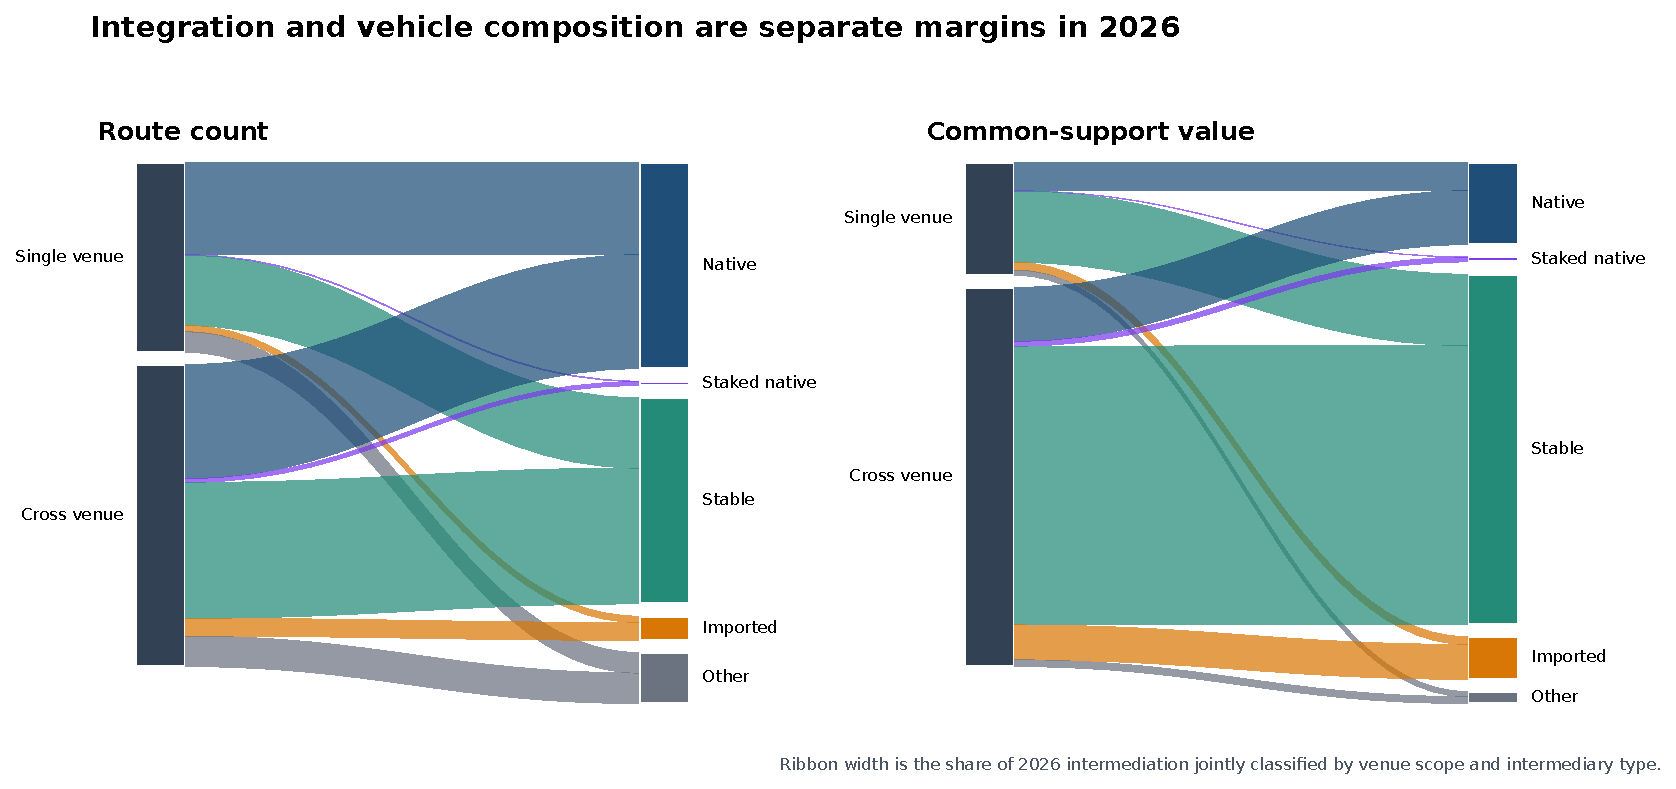
\includegraphics[width=0.93\textwidth,height=0.66\textheight,keepaspectratio]{../output/figures/experiments/integration_vehicle_alluvial.pdf}
\end{center}
\vspace{-0.12cm}
{\scriptsize The ribbons classify realised intermediation jointly by venue scope and intermediary type. They describe selected routes; they do not identify an effect of integration or the unchosen opportunity set.\par}
\vfill
\end{frame}

% VISUAL-FUNCTION: intellectual provenance | grouped reference list | support vehicle-currency and market-structure framing
\begin{frame}{A12. References: vehicle currencies and market structure}
\begin{itemize}
\item Amiti, Itskhoki and Konings (2022), \emph{Quarterly Journal of Economics}
\item Dowd and Greenaway (1993), \emph{Economic Journal}
\item Flandreau and Jobst (2009), \emph{Economic Journal}
\item Gopinath and Stein (2021), \emph{Quarterly Journal of Economics}
\item Krugman (1980), \emph{Journal of Money, Credit and Banking}
\item Makarov and Schoar (2020), \emph{Journal of Financial Economics}
\end{itemize}
\end{frame}

% VISUAL-FUNCTION: institutional provenance | grouped reference list | support AMM architecture and liquidity design
\begin{frame}{A13. References: decentralised exchange design}
\begin{itemize}
\item Adams et al. (2021), \emph{Uniswap v3 Core}
\item Angeris, Chitra, Evans and Boyd, optimal routing in constant-function markets
\item Barbon and Ranaldo, decentralised exchange costs and market structure
\item Lehar and Parlour (2024), \emph{Journal of Finance}
\item Milionis, Moallemi, Roughgarden and Zhang, loss versus rebalancing
\item Xu, Paruch, Cousaert and Feng, AMM design and slippage
\end{itemize}
\end{frame}


\end{document}
